\chapter[Some Mathematical Aspects of Three-Dimensional.....]{Some Mathematical Aspects of Three-Dimensional
  Elasticity}\label{chap2}\pageoriginale 

IN THIS CHAPTER, questions of existence of solutions to the boundary
value of three-dimensional elasticity will be examined. In the first
section, some general considerations about these boundary value
problems will be mentioned. The problems will be classified with
respect to boundary conditions. As good models of elasticity must
preclude uniqueness of solution, several examples of non-uniqueness
will be presented.  

The first tool for the study of existence of solutions is the implicit
function theorem. As this requires a knowledge of the linearized
problem, the second section will briefly present linear elasticity and
the third section will prove existence, albeit for a very narrow class
of boundary conditions. The fourth section will study incremental
methods, whose analysis follows closely related lines.  

The last two sections will present results on polyconvexity and
existence of solutions to the problem of minimizing the energy using
the approach of J. BALL. Though several types of boundary conditions
can be studied here, the main drawback is the lack of regularity of
solutions and so it is not known if the solutions satisfy the
equilibrium equations.
  
\section[General Considerations\ldots]{General Considerations About
  the Boundary\break Value Problems of 
  Three-Dimensional Elasti\-city}\label{chap2-sec2.1}\pageoriginale 

\markright{2.1. General Considerations\ldots}

Given a respones function $\hat{T}_R : \mathbb{M}^3_+ \to
\mathbb{M}^3$ satisfying 
\begin{equation*}
  F (\hat{T}_R (F))^T = \hat{T}_R (F)F^T \tag{2.1-1}\label{eq2.1-1}
\end{equation*}
for every $F \epsilon \mathbb{M}^3_+$ and given the denstiy $\rho_R
: \mathcal{B}_R \to \mathbb{R}$ and dead loads $b_R : \mathcal{B}_R
\to \mathbb{R}^3, \imath_{\mathbb{R}} :\partial \mathcal{B}_{1R} \to
\mathbb{R}^3$, the boundary value problem arising out of the
equilibrium equations amounts to finding a deformation $\Phi$ which
satisfies 
\begin{gather*}
  DIV_R \hat{T}_R (\nabla \phi) + \rho_R b_R = 0 ~
  \text{in}~\mathcal{B}_R \tag{2.1-2}\label{eq2.1-2} \\
 \hat{T}_R (\nabla \phi)n_{\mathbb{R}} = t_{1R} ~\text{on}~
 \partial \mathcal{B}_{1R} \tag{2.1-3}\label{eq2.1-3} \\
\phi = \phi_o ~\text{(given) on}~ \partial \mathbb{B}_{oR}
\tag{2.1-4}\label{eq2.1-4}
\end{gather*}

The boundary condition $\phi = \phi_o $ on $\partial \mathbb{B}_{oR}$
is called a {\em boundary condition of place}.\index{boundary
condition of place} The boundary condition
\eqref{eq2.1-3} on $\partial \mathbb{B} _{1R}$ is called a {\em
  boundary condition of traction}\index{boundary condition of
  traction} (and this defnition implies it is a dead load).  

If $\partial \mathcal{B}_{oR} = \phi$ the problem is a {\em pure
traction}\index{pure traction problem}
boundary value problem.If $\partial \mathcal{B} _{1R}$ the problem is
a {\em pure displacement} problem.\index{pure displacement problem} If both $\partial \mathcal{B}_{oR}$ and
$\partial \mathcal{B}_{1R} $ have strictly positive $dA_R$- measure,
then the problem is a {\em mixed displacement-tranction}\index{mixed displacement-tranction problem} problem. 

Recall that
$$
\displaylines{\hfill
  \hat{\sum}_R (\nabla \phi) = (\nabla \phi) ^{-1}
  \hat{T}_R (\nabla \Phi)\hfill \cr
  \text{where}\hfill
  \hat{\sum}_R : \mathbb{M}^3_+ \to \mathbb{S}^3\hfill}
$$\pageoriginale
and the boundary value problem \eqref{eq2.1-2}--\eqref{eq2.1-4} can be
rewritten in 
terms of this tensor. If the material is hyperelastic (cf. Section
\ref{chap1-sec1.4}), then 
\begin{equation*}
  \hat{T}_R (F) = \frac{\partial \mathcal{W}} {\partial F} (F)
  \tag{2.1-5}\label{eq2.1-5} 
\end{equation*}
for a stored energy function $\mathcal{W} : \mathbb{M}^3_+ \to
\mathbb{R}$ and the problem is equivalent to finding the sationary
points of an energy functional, 
\begin{equation*}
  I (\psi) = \int \limits_{{\mathcal{B}}{_R}} \mathcal{W}
  (\nabla \psi) dX_R - \left(\int\limits_{{\mathcal{B}}{_R}} \rho_R
  b_R. \psi dX_R + \int\limits_{{\partial \mathcal{B}} _{1R}}
  t_{1R}. \psi dA_R \right) \tag{2.1-6} \label{eq2.1-6}
\end{equation*}
 
 The partial differentail equations \eqref{eq2.1-2} are nonliner with respect
 to $\phi$ since the mapping $\hat{T}_R : \mathbb{M}^3_+ \to
 \mathbb{M}^3$ is non-linear, and of the second order. The
 non-linearity occurs in the highest order terms and this is a source
 of difficulty. Another source of difficulty is that the solution
 $\phi$ must satisfy det $(\nabla \phi) > o$. Thus for instance
 in \eqref{eq2.1-6} $\psi$ must vary over $\mathbb{M}^3_+$ which is clearly not
 a vector sapce; in fact it is not even a convex subset of
 $\mathbb{M}^3$ (cf. Exercise 1.4-2). 
 
 The boundary condition of traction could be replaced by the so-called
 {\em boundary condition of pressure}\index{boundary condition of
 pressure} (which is not a dead load, but it is 
 conservative). Again it is possible to have a {\em pure pressure} boundary
 value problem\index{pure pressure problem} (for instance, a soap bubble or a submarine) or {\em mixed
 displacement-pressure}\index{mixed displacement-pressure problem} boundary value problems. 
 
 These boundary condition, though being the only ones to be
 considered here, are far from exhaustive. Other types of conditions
 are possible. 
 
 In\pageoriginale practice one can have {\em unilateral
   conditions}.\index{unilateral boundary condition} For instance, if the 
 body must remain in above the plane spanned by $e_1,e_2$ the boundary
 condition is $X_3 \geq o$ or $\phi_3 (X_R) \geq o$  
 
\setcounter{figure}{0}
\begin{figure}[H]
\centering
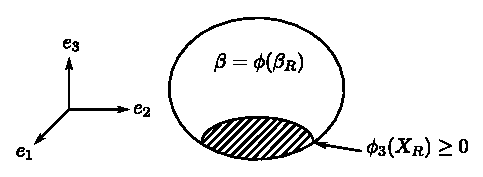
\includegraphics{vol71-figures/fig2.1-1.eps}
\medskip
\caption{}\label{fig2.1.1}
\end{figure}

It is also possible to have a mixture of displacement and stress boun\-dary
conditions. Consider $\mathcal{B}_R$ to be a plate with a pressure $p$
compressing the lateral surface (fig~\ref{fig2.1.2}) and given only by its
{\em horizantal average}. Then the conditions are  
\begin{equation*}
  \begin{cases}
    u_1, u_2 \text{independent of} X_3\\
    u_3 = 0 \tag{2.1-7}\label{eq2.1-7}
  \end{cases}
\end{equation*} 
 and
\begin{equation*}
   \frac{1}{2 \epsilon} \int\limits_{-\epsilon}^{\epsilon} T
   (\nabla \phi (X_R)n~ dX_3 = -pn. \tag{2.1-8} \label{eq2.1-8}
\end{equation*} 
 
\begin{figure}[H]
\centering
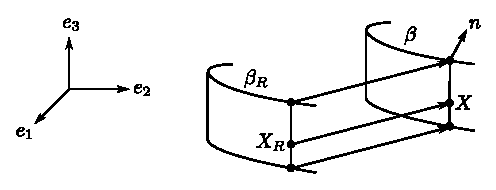
\includegraphics{vol71-figures/fig2.1-2.eps}
\medskip
\caption{}\label{fig2.1.2}
\end{figure}\pageoriginale

Apart from possibly the problem of bodies moving with constant
velocity in a fluid, the pure traction problems are less common. The
pure displacement problems are quite unrealistic. 

In general, several deformed states are possible for the same system
of forces, though they may not all be physically feasible or `stable'.
Nevertheless the mathematical model cannot recognize the feasible or
stable ones. Hence a good model will always account for non-uniqueness
of solutions. Several examlpes of non-uniqueness will now be given . 

\begin{example}\label{chap2-exam2.1.1}% example 2.1-1
A mixed displacement-traction problem. Consider a long circular
cylinder fixed at either end. The body force is just its weight. On
the lateral surface $t_{1R} = o$. Assume the body to be extremely
pliable, and rotate one end by an angle of $2 \pi$ and reglue it in
its original position. Then a line parallel to the axis on the lateral
surface will deform into a curve and thus gives another solution\pageoriginale other
than the natural one, which will just be a slight bending of the
cylinder under its weight. It is theoretically possible to rotate the
face by $2 k \pi$ for any positive integer $k$. Thus the model must
account for an infinite number of solutions.  

\begin{figure}[H]
\centering
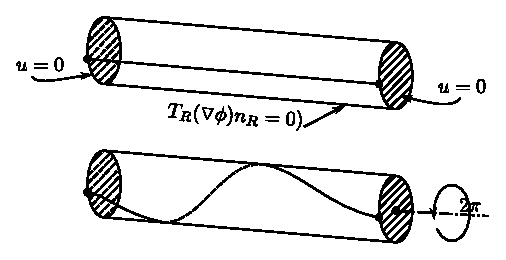
\includegraphics{vol71-figures/fig2.1-3.eps}
\medskip
\caption{}\label{fig2.1.3}
\end{figure}
\end{example}

\begin{example}[F.~JHON]\label{chap2-exam2.1.2} % example 2.1-2
   A pure displacement problem. Consider the body to be
  betwen two concentric spheres. Assume $u \equiv 0$ on both the inner
  and outer surfaces. Apart from the trivial solution, it is possible
  to have an infinite number of solutions by (theoretically) rotating
  the inner sphere about an axis by an angle of $2 k \pi$ and
  re-glueing it to the body.  
\begin{figure}[H]
\centering
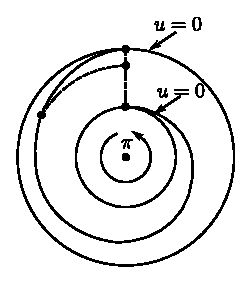
\includegraphics{vol71-figures/fig2.1-4.eps}
\medskip
\caption{}\label{fig2.1.4}
\end{figure}\pageoriginale
\end{example}

\begin{example}[C. ERICKSEN]\label{chap2-exam2.1.3}% example 2.1-3
   A pure traction problem.A rectangular lock is pulled
  normal to the upper and lower surfaces. Rotation of the
  configuration by $\pi$ produces a (though urrealistic) solution
  where the body is comprssed! 
\begin{figure}[H]
\centering
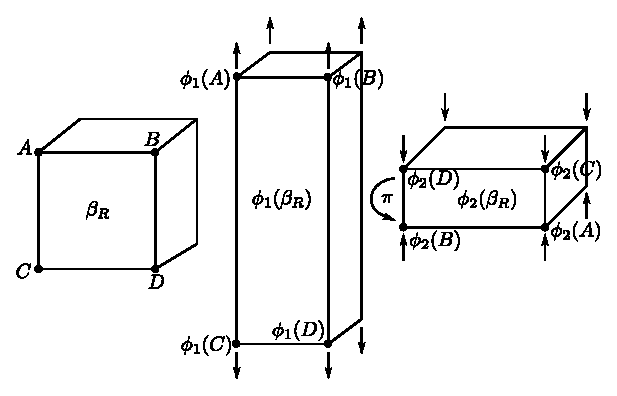
\includegraphics{vol71-figures/fig2.1-5.eps}
\medskip
\caption{}\label{fig2.1.5}
\end{figure}
\end{example}

\begin{example}\label{chap2-exam2.1.4}% 2.1-4
 Consider\pageoriginale a thin circular plate subjected to the
 boundary condition 
  \eqref{eq2.1-7} - \eqref{eq2.1-8} with $p = \lambda p_1$. If
  $\lambda < 0$ (i.e the 
  plate is pulled) or if $\lambda > o$ and small, $u \equiv o$ is the
  only possible solution. If $\lambda$ exceeds a critical value, the
  plate can buckle upwards or downwards thus giving two additional
  solutions (cf. \ref{fig2.1.6}) This is a buckling phenomenon 
\end{example}


\begin{example}\label{chap2-exam2.1.5}% example 2.1-5
  Eversion problems. A cut tennis ball (borrowed from a very good
  friend) can be made to exist in two diffrent states as shown in 
fig~\ref{fig2.1.7}. The everted state can be produced by pushing
hard\pageoriginale enough on 
  the natural state. 
\begin{figure}[H]
\centering
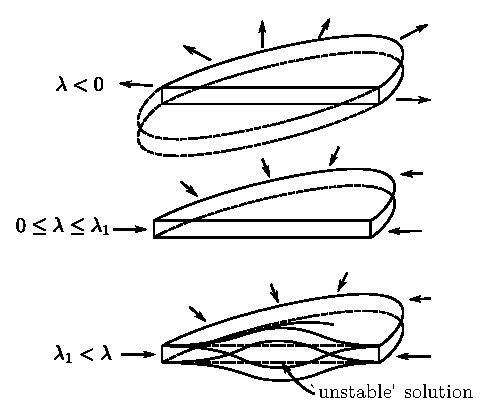
\includegraphics{vol71-figures/fig2.1-6.eps}
\medskip
\caption{}\label{fig2.1.6}
\end{figure}

\begin{figure}[H]
\centering
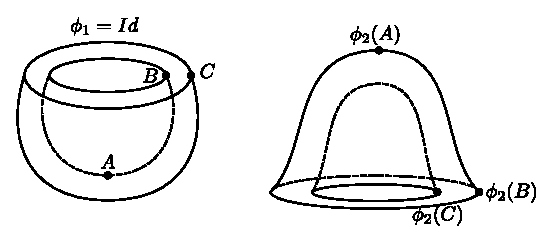
\includegraphics{vol71-figures/fig2.1-7.eps}
\medskip
\caption{}\label{fig2.1.7}
\end{figure}


It is possible to do the same thing to a tube. These are examples of
multiple solutions to a pure traction problem. 
\end{example}

Returning to the various restrictions on the model and its analysis,
the first is the taking into account of properties like isotropy,
hyperelasticity and the axiom of material frame indifference. These
are fairly easy to handle. In sections \ref{chap1-sec1.3} and
\ref{chap1-sec1.4}  various
necessary and sufficient conditions of the relevant functions were
studied. The main restriction is that the solution $\phi$ must satisfy
forces 
$$
\det (\nabla \phi) > o.
$$

In using the implicit function theorem, this requirement is ignored at
first and then shown to be satisfied for sufficiently small forces. 

In\pageoriginale the different approach of J. BALL, this is taken into
account (a.e 
in $\mathcal{B}_R$) by imposing it on the set $\mathscr{U}$ of test
functions over which the energy is minimized. This precludes the
convexity of $\mathscr{U}$ which makes minimization more difficult
than usual. In this approach, it will be nicely taken into account by
imposing that $\mathcal{W} (F) \to + \infty$ when det $(F) \to o^+$.  
 
 Even if $\det \nabla \phi > o$ everywhere on
 $\mathcal{B}_R$, it does not ensure that $\phi$ is a one-one mapping,
 a property natural to expect in a deformation.Thus if a body as in
 fig.~\ref{fig2.1.8}(a) in contact with the horizontal plane is pushed along
 the two `arms', it must take a shape as in fig~\ref{fig2.1.8}(b). But the
 mathematical model will not preclude a situation as in fig~\ref{fig2.1.8}(c)
 where the material penetrates itself, still keeping det
 $\nabla \phi > 0$ 

\begin{figure}[H]
\centering
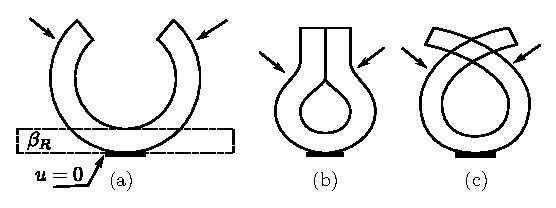
\includegraphics{vol71-figures/fig2.1-8.eps}
\medskip
\caption{}\label{fig2.1.8}
\end{figure}

In\pageoriginale the case of incompressible materials, the energy is
minimized over 
a set of function $\psi$ (in a suitable function space) with 
$$
\det (\nabla \psi) =1 ~\text{a.e}.
$$

Some of the noations used hitherto will be changed. $\mathfrak{B} _R$
will henceforth be denoted by $\bar{\Omega}, \Omega$ a bounded open
subset of $\mathbb{R}^3$ and its boundary $\partial \mathfrak{B} _R$
by $\Gamma$. The portions $\partial \mathfrak{B} _{oR} \text {and}
\partial \mathfrak{B}_{1R}$ will be denoted by $\Gamma_o$ and
$\Gamma_1$ respectively. 

The generic point $X_R$ will henceforth be labelled $x$ and $dX_R
~\text{and}~dA_R$ will be changed to $dx$ and $da$ respectively. The
derivatives $\dfrac{\partial}{\partial X_{Ri}}$ will be denoted by
$\partial_i$ and $DIV_R$ by div. The normal $n_R$ to
$\partial\mathfrak{B}_R$ will now be given by $v=(v_i)$, the unit
outer normal to $\Gamma$. 

The tensors $\sum\limits_R = (\sum\limits_{R_{ij}})$ and $T_R =
(T_{R_{ij}})$ will be denoted by $(\sigma_{ij}) $ and $(t_{ij})$
respectively. The vectors $\rho_Rb_R$ and $t_{1R}$ will be denoted by
$f=(f_i)$ and $g = (g_i)$ respectively. The symbols for $\phi , u, F=
\nabla \phi, B= FF^T, C= F^T $ and $E=\dfrac{1}{2} (C-I)$
will remain unchanged. 

Thus, for instance the equations of equilibrium im terms of $\sum_R$
read in the old natation as: 
\begin{align*}
  \text{DIV}_R \left(\nabla\phi \sum_R\right)+\sigma _R b_R & = o
  ~\text{in}~ \mathfrak{B} _R\tag{2.1-9}\label{eq2.1-9}\\  
  \nabla \phi \sum_R n_R &= t_{1R} ~\text{on}~
  \partial\mathfrak{B}_{1R}\tag{2.1-10}\label{eq2.1-10}\\ 
  \phi &=\phi_0 ~\text{on}~ \partial
  \mathfrak{B}_{0R}\tag{2.1-11}\label{eq2.1-11} 
\end{align*}

These,\pageoriginale when translated in to the new notations will read as 
\begin{align*}
  - \partial_j (\sigma_{kj}\partial_k \phi_i)&= f_i ~\text{in}~
  \Omega\tag{2.1-12}\label{eq2.1-12}\\ 
  \sigma_{kj}\partial_{k}\phi_iv_j &= g_i ~\text{on}~
  \Gamma_1\tag{2.1-13}\label{eq2.1-13}\\ 
  \phi_i &=\phi_{0i} ~\text{on}~ \Gamma_0\tag{2.1-14}\label{eq2.1-14}
\end{align*}

\medskip
\begin{center}
{\large\bf Exercises}
\end{center}

\begin{description}
\item[2.1-1]. Assume that a pure traction problem has a solution
  $\phi$. Show that  
$$
\displaylines{\hfill
  \int\limits_{\mathfrak{B}_R} \rho_R b_R dX_R + \int\limits_{\partial
  \mathfrak{B}_R} t_{1R} dA_{R}=0 \hfill\cr
  \text{and}\hfill 
  \int\limits_{\mathfrak{B}_R} \phi \Lambda \rho_{R} b_R dX_R +
  \int\limits_{\partial \mathfrak{B} _R} \phi \Lambda t_{1R} dA_R
  =0.\hfill} 
$$


\item[2.1-2] .Consider a hyperelastic
  incompressible\index{material!incompressible} 
  material.\index{incompressible material} In the
  constrained minimization problem 
$$
\displaylines{\hfill
\inf\limits_{\psi \epsilon \mathcal{U}} I(\psi)\hfill\cr
\text{where}\hfill  
\mathcal{U}=\{\psi \mid \det \left(\nabla \psi\right) =1
\text{a.e.}\},\hfill} 
$$ 
show by a formal computation that the Lagrange multiplier is the pressure.
\end{description}

\section{The Linearized System of Elasticity}\label{chap2-sec2.2}%sec
\index{linearized system of elasticity}\pageoriginale                                %2.2\pageoriginale 
\setcounter{figure}{0}

Consider the boundary value problem
\eqref{eq2.1-12}-\eqref{eq2.1-14}. In terms of the displacement $u$ it
can be rewritten as   
\begin{align*}
-\partial_j(\sigma _{ij}+\sigma_{kj} \partial_{k} u_i) &= f_i
~\text{in}~\Omega,\tag{2.2-1}\label{eq2.2-1}\\ 
(\sigma_{ij}+\sigma_{kj} \partial_k u_i) v_j &= g_i ~\text{on}~
\Gamma_1,\tag{2.2-2}\label{eq2.2-2}\\ 
u_i &=u_{oi} ~\text{on}~ \Gamma_o,\tag{2.2-3}\label{eq2.2-3}
 \end{align*}
with the constitutive equation 
\begin{equation*}
 \sigma_{ij} = \sigma^*_{ij} (E(u)) = \lambda
 E_{kk}(u)\delta_{ij}+2\mu E_{ij} (u)+o(E)\tag{2.2-4}\label{eq2.2-4}  
\end{equation*}
where
\begin{equation*}
E(u)=\frac{1}{2} \left(\nabla u^T + \nabla u +
\nabla u^T \nabla
u\right)\tag{2.2-5}\label{eq2.2-5} 
\end{equation*}

If $u$ were defined in a suitable function space, whose functions
vanish on $\Gamma _0$, then symbolically one can write 
\begin{equation*}
  A(u)=\begin{bmatrix} 
  f \\ 
  g 
  \end{bmatrix}\tag{2.2-6}\label{eq2.2-6}
\end{equation*}

The linearised system of elasticity will then be formally defined as
(assuming $A$ is differentiable) 
$$
  A'(0)u=
  \begin{bmatrix} 
    f \\ 
    g 
  \end{bmatrix}
$$

This can be derived as follows. The linearized strain
tensor\index{linearized strain tensor}\index{strain!linearized -tensor} is  
\begin{equation*}
  \epsilon (u)=\frac{1}{2}\left(\nabla u^T + \nabla
  u\right).\tag{2.2-7} \label{eq2.2-7}
\end{equation*}

Then $\sigma$ will in turn be linearized as 
\begin{equation*}
  \sigma_{ij} = \lambda \epsilon_{kk}(u) \delta_{ij} + 2\mu
  \epsilon_{ij} (u).\tag{2.2-8} \label{eq2.2-8}
\end{equation*}\pageoriginale

Substituting this in \eqref{eq2.2-1}-\eqref{eq2.2-3} and keeping only
the first order 
terms, the linearized syatem elasticity turns out to be  
\begin{align*}
  -\partial_{j} \sigma_{ij} &=f_i \text{ \ in\ }
  \Omega\tag{2.2-9}\label{eq2.2-9}\\ 
  \sigma_{ij} v_j &= g_i \text{ \ on\ } \Gamma_1\tag{2.2-10}\label{eq2.2-10}\\
  u_i &= u_{oi} \text{ \ on\ } \Gamma_0\tag{2.2-11}\label{eq2.2-11}
 \end{align*} 
 where $\sigma$ is given by \eqref{eq2.2-8}. Note that such a syatem
 cannot be 
 a model for elasticity (of Exercise 2.2-1) but only approximation
 of a model. 
 
 \begin{remark}\label{chap2-rem2.2.1} % remark 2.2-1
   If the equations were written in terms of $t_{ij}$ and then
   linearized, the same linearized system of elasticity would have
   been obtained. This is because $T_R= (I+ \nabla u)
   \sum\limits_R$ and on linearizing this realtion only the part
   coming from $I\sum\limits_R = \sum\limits_R$ will be retained. 
 \end{remark}
 
 Before the existence and regularity of solution to the linearized
 system of elasticity can be studied the following notations for the
 Sobolev spaces will be needed. 
 
Let $m \geq 0$ be an integer and $1 \leq p \leq + \infty$. Then 
 \begin{equation*}
   W^{m,p}(\Omega) = \{v \epsilon L^p (\Omega)\mid \partial^\alpha
   v \epsilon L^p (\Omega) \text{for all} \mid \alpha \mid \leq m
   \} \tag{2.2-12} \label{eq2.2-12}
\end{equation*}
where $\alpha$ is a multi-index and $\partial^\alpha v$ is the
 corresponding partial derivative ( in the sense of
 distribution). This space is a Banach space with the norm   
 \begin{equation*}
 \mid \mid v \mid \mid _{m, p.\Omega} = \left(\int\limits_\Omega \sum_{\mid
   \alpha \mid \le m} \mid \partial^\alpha v \mid ^p
 dx\right)^{1/p}\tag{2.2-13} \label{eq2.2-13}
 \end{equation*}\pageoriginale
  (with the standrad modification if $p=+\infty$). The semi-norm
 $\mid. \mid_{m, p, \Omega}$ is defined by   
  \begin{equation*}
    \mid \mid v \mid \mid _{m, p.\Omega} = \left(\int\limits_\Omega \sum_{\mid
      \alpha \mid = m} \mid \partial^\alpha v \mid ^p
    dx\right)^{1/p}\tag{2.2-14} \label{eq2.2-14}
  \end{equation*} 
  
 If $m=0, W^{0,p}(\Omega)= L^p (\Omega) \text{and} \mid .\mid _{0, p,
   \Omega}$ is the usual $L^p(\Omega)$- norm. If $\mathscr{D}(\Omega)$
 is the space of $C^\infty$ functions with compact support in
 $\Omega$, its closure in $W^{m ,p} (\Omega)$ will be denoted by
 $W^{m,p}_o(\Omega)$.  
  
 If $p=2$, it is customary to write $H^m(\Omega)
 \text{and}H^m_0(\Omega)$ instead of $W^m$, $2(\Omega)$
 and $W^{m,2}_0(\Omega)$ respectively. The norms and semi-norms
 in this case will be written as $\mid \mid \cdot \mid \mid _{m, \Omega}$
 respectively $| \cdot | _{m, \Omega}$ is the $L^2(\Omega)$- norm. 
 
 By Poincar\'es inequality, $\mid \cdot \mid _{m,p,\Omega}$ is a norm on
 $W^{m.p}_0(\Omega)$ and is equivalent to $\mid \mid . \mid \mid
 _{m,p\Omega}, \text {for} 1\leq p < \infty$. 
 
 In case of vector valued or tensor valued functions, the symbols
 $W^{m,p}(\Omega)$, $\mathbb{L}^P(\Omega)$ will be used to denote that
 each component is in $W^{m,p}$ $(\Omega)$ or $L^p(\Omega)$
 respectively. However the symbols for the norms and semi-norms will
 not be altered.  
 
 The following result is fundamental.
  
 \begin{theorem}[Korn's Inequality]\index{Korn's inequality}% them{2.2-1}
    Let $\Gamma$ be smooth enough. Then
    \begin{equation*}
      \{v=(v_i)\epsilon \mathbb{C}^2(\Omega)\mid \epsilon_{ij}(v)
      \epsilon L^2(\Omega), 1 \leq i,j\leq 3\} = 
      \mathbb{H}^1(\Omega)\tag{2.2-15} \label{eq2.2-15}
  \end{equation*}

    Consequently,\pageoriginale there exists constans $C_1 > 0 \text
    {and} C_2 > 0$ such that 
  \begin{equation*}
    C_1 \mid \mid v \mid \mid _{1,\Omega} \le (\mid v \mid ^2_{0,
      \Omega}+ \mid \epsilon (v) \mid ^2_{0,\Omega})^{1/2} \le C_2
    \mid \mid v \mid \mid _{1,\Omega}\text{for all} v \epsilon H^1
    (\Omega).\tag{2.2-16} \label{eq2.2-16}
  \end{equation*}
\end{theorem} 
  
\begin{proof}
  See DUVAUT and LIONS [1972] or NITSCHE [1981]. The main
  difficulty is in proving \eqref{eq2.2-15}. Since the second inquality of
  \eqref{eq2.2-16} is obvious, the first follows from \eqref{eq2.2-15}
  and the closed graph theorem. 
\end{proof} 
  
A consequence of the above result is
 
\begin{theorem}\label{chap2-thm2.2.2}% them 2.2-2
  Let $\mathbb{V}$ be defined by 
\begin{equation*}
  \mathbb{V} = \{v \epsilon \mathbb{H}^1 (\Omega) \mid v =0
  ~\text{on}~ \Gamma_0\}\tag{2.2-17}\label{eq2.2-17} 
 \end{equation*} 
 where the da-measure of $\Gamma_0$ is strictly positive. Then the
 semi-norm $\mid \epsilon (v)\mid _{0, \Omega}$ is a norm on $V$
 equivalent to the norm $\mid \mid . \mid \mid _{1,\Omega}$.  
\end{theorem}

\begin{proof}
Cf. Exercise~2.2-2.
\end{proof}

Assume now that $u=0$ on $\Gamma_0$. Let $V$ be as in
\eqref{eq2.2-17}. Multiplying \eqref{eq2.2-9} by a function $v \epsilon
\mathbb{V}$, integration by parts using Green's formula, and using
\eqref{eq2.2-10}, \eqref{eq2.2-11} and the symmetry of $\sigma$, the following
variational formulation of the problem \eqref{eq2.2-9} -
\eqref{eq2.2-11} can be obtained. 
   
  
 Find $u \epsilon \mathbb{V}$ such that, for all $v \epsilon
 \mathbb{V}$, 
\begin{equation*}
a(u, v) = L(v) \tag{2.2-18}\label{eq2.2-18}
\end{equation*}
where
\begin{equation*}
a (u, v)= \int\limits_{\Omega} (\lambda\epsilon_{kk}
    (u)\epsilon_{\ell\ell}(v)+ 2\mu\epsilon_{ij} (u)
    \epsilon_{ij} (v)) ~ dx \tag{2.2-19}\label{eq2.2-19}
\end{equation*}
and
\begin{equation*}
L(v)=\int\limits_{\Omega} f_i v_i dX + \int\limits_{\Gamma_1} g_i v_i
    ~ da.\tag{2.2-20}
\end{equation*}\pageoriginale
  
 By a simple application of Schwarz's inequality, it follows that
 $a(.,.)$ is a continuous bilinear form on $\mathbb{H}^1(\Omega)$ and
 $L$ is a continuous functional on $\mathbb{H}^1(\Omega)$ (and hence on
 $\mathbb{V}$ as well). 


The following existence result holds. 
  
\begin{theorem}\label{chap2-thm2.2.3}% them 2.2-3
Consider the variatiational formulation of the linea\-rized syatem of
elasticity, \eqref{eq2.2-18}, or, equivalently, the problem: Find $u
\epsilon \mathbb{V}$ such that 
\begin{equation*}
J(u)=\inf\limits_{v \epsilon \mathbb{V}} J(v) \tag{2.2-21}\label{eq2.2-21}
\end{equation*}
where
\begin{equation*}
J(v)=\frac{1}{2} a (v,v) - L(v)\tag{2.2-22}\label{eq2.2-22}
\end{equation*}
if $\lambda > 0$ and $\mu > 0$ then the problem has a unique solution.
\end{theorem} 
  
\begin{proof}
Observe that by Theorem~\ref{chap2-thm2.2.2} for all $v \epsilon
\mathbb{V}$, 
\begin{equation*}
  a(v,v) \ge 2\mu \mid \epsilon (v) \mid ^2_{0,\Omega} \ge \alpha
  \mid \mid v \mid \mid ^2_{1,\Omega} \tag{2.2-23} \label{eq2.2-23}
\end{equation*}
where $\alpha > o$ (using $\lambda > o$ and $\mu > o$). Thus $J:
\mathbb{V}\to \mathbb{R}$ is a convex, and continuous
functional. Hence it is weakly lower semi continuous. Let $\{u_k\}$ be
a minimizing sequence in $\mathbb{V}$, i.e. 
$$
J(u_k)\to \inf\limits_{v \epsilon \mathbb{V}} J(v) < + \infty.
$$

Since $J$ is coercive (i.e., $J(v) \to \infty \text{as}\mid \mid v \mid
\mid \to \pm \infty )$ it follows that $\{u_k\}$ is a bounded sequence
and hence has a weakly convergent subsequence.\pageoriginale Let $u$ be the weakly
limit of the subsequence (again indexed by $k$ for convenience). Then
by the weak lower semi-continuity of $J$. 
$$
\inf\limits_{v \epsilon \mathbb{V}} J(v)\le J(u) \le
\lim\limits_k\inf\limits_{\to \infty} J(u_k)= \inf\limits_{v \in
  \mathbb{V}} J(v). 
$$

Thus $J$ attains its mimimum at $u$. It is easy to see that equations
\eqref{eq2.2-18} are simply equivalent to the equation $J'(u)=0$. Hence the
equivalencve of the two problems since $J$ is convex and the existence
of a solution. 

If $u_1$ and $u_2$ are solutions in $\mathbb{V}$ then $a(u_1-u_2,
v)=0$ for all $v \epsilon \mathbb{V}$. Setting $v=u_1-u_2$ and
using \eqref{eq2.2-23}, it follows that $u_1 = u_2$, thus proving the
uniqueness of the solution. 
\end{proof}

\begin{remark}\label{chap2-rem2.2.2}% rem 2.2-2
  The existence of a unique solution to \eqref{eq2.2-18} also follows directly
  from \eqref{eq2.2-23} by applying the {\em Lax-Milgram Lemma.} 
\end{remark}

Finally, let us state the result on the regularity of solutions to the
above problem. 

\begin{theorem}\label{chap2-thm2.2.4}% them 2.2-4
  Suppose $\Gamma$ is smooth enough and for some $p \ge 2$,\break $f
  \epsilon \mathbb{C}^p (\Omega)$. Assume $\Gamma_1= \phi$. Then
  the solution $u \epsilon \mathbb{V} = \mathbb{H}^\imath_0 (\Omega)$ of
  the corresponding linearized system of elasticity is in the space
  $\mathbb{V}^p(\Omega)$, where  
  \begin{equation*}
    \mathbb{V}^p(\Omega) = \{v \epsilon \mathbb{W}^{2,p}(\Omega)
    \mid v = 0 ~\text{on}~ \Gamma\}.\tag{2.2-24} \label{eq2.2-24}
  \end{equation*}
\end{theorem}

\begin{proof}
  The case $p=2$ has been proved by NE\v{C}AS [1967]. If $p > 2$, the
  argument goes as follows. Let $A'(0):\mathbb{V}^p(\Omega)\to
  \mathbb{C}^p (\Omega)$ represent the operator of the linearized
  system of elasticity. Then, if index $(A' (0))\overset{\de}{=}\dim
  (\ker A' (0))-\dim (Coker A' (0))$, it was proved by GEYMONAT\pageoriginale
  [1965] that for all $p, 1< p< \infty $, the index was independent
  of $p$. Now, by the result of Necas above if $p=2, A'(0)$ is onto
  and so $\dim (Coker (A'(o)) = 0$. By uniqueness of the solution,
  $\dim (ker (A'(0))=0$ for all $ p \ge 2$. Hence the index is zero
  for all $p$ and so $\dim (Coker(A'(o)))=0$ for all $p \ge 2$,
  i.e., $A'(0)$ is onto for all $p \ge 2$, which proves the theorem. 
\end{proof}

\begin{remark}\label{chap2-rem2.2.3}% rem 2.2-3
  The above result does not follow from those of AGMON, DOUGLIS and
  NIRENBERG [1964]. Their results state that if $f \epsilon
  \mathbb{L}^p(\Omega)$ implise $u\epsilon\mathbb{W}^{2,p}(\Omega)$
  then $f \epsilon \mathbb{W}^{m,p}(\Omega)$ implies $u
  \epsilon\mathbb{W}^{2+m,p}(\Omega)$ for our problem. The
  'starting' regularity result $(m=0)$ needs be know a priori and
  Theorem \ref{chap2-thm2.2.4} proves that in case of the linearized
  syatem of elasticity. 
\end{remark}

Caution! The $W^{2,p}$ regularity does not hold for the mixed
displace\-ment-traction linearized syatem of elasticity. 

\medskip
\begin{center}
{\large\bf Exercises}
\end{center}

\begin{description}
\item[2.2-1] Show that if $\epsilon(u)=
  \dfrac{1}{2}(\nabla u^T + \nabla u)$, then a
  constitutive equation of the form $\sigma = \sigma^*(\epsilon)$,
  with $\sigma^*$ a linear function of $\epsilon$, does not satisfy
  the axion of material frame indenfference. 

\item[2.2-2] Prove Theorem $2.2-2$. (Show first that $|\epsilon
  (v)|_{0\Omega}$) is a norm on $\mathbb{V}$. Prove the equivalence of
  norms by contradiction: assume there exists a sequence $v^k
  \epsilon\mathbb{V}$ with $|| v^k ||_{1,\Omega}=1 $ and
  $|\epsilon (v^k)|_{0,\Omega} \to 0$. 

\item[2.2-3] Consider the
  linearized system of elasticity in variational form with $\Gamma_0=
  \phi$. Show that there exists a solution to the problem provided 
$$
\int\limits_{\Omega} f ~ dx = \int\limits_{\Gamma} ~ dx,
$$\pageoriginale
in the quotient space $H^1(\Omega)\mathbb{W}$, where 
$$
\mathbb{W} = \{v \epsilon \mathbb{H}^1(\Omega) \mid \epsilon
(v)=0\}. 
$$

Show also that 
$$
\mathbb{W} = \{v \epsilon | \mathbb{H}^1 (\Omega)| v = a+b ~\Lambda~
ox\}.  
$$ 

\item[2.2-4] Extend the regularity result to the case $1 < p < 2$. 

\item[2.2-5] Show that if $\mu > 0$, there exists a $\lambda_0 < 0$
  such that if $\lambda_0 < \lambda \le 0$, the linear form $a(.,.)$
  given by \eqref{eq2.2-19} is coercive. 
\end{description}

\section{Existence Theorems via Implicit Function
  Theorem}\label{chap2-sec2.3}
\setcounter{figure}{0}

In this section, existence solutions to the {\em pure displacement
  problem}\index{pure displacement problem} will be proved using the implict function theorem. 

For simplicity, consider first a St Venabt-Kirchhoff\index{material!St Venant-Kirchhoff}\index{St Venant-Kirchhoff material} marerial Recall 
that the constitutive equation in this case can be written as  
\begin{equation*}
  \sigma_{ij} = a_{ijk\ell}\, E_{k\ell} (u) = \lambda E_{kk} (u)
  \delta_{ij} + 2\mu E_{ij}(u), \tag{2.3-1}\label{eq2.3-1} 
\end{equation*}
with $\lambda > 0$ and $\mu > 0$. Also
\begin{equation*}
  E_{ij}(u)=\epsilon_{ij} (u) + \frac{1}{2} \partial_i u_m \partial_j
  u_m,\tag{2.3-2}\label{eq2.3-2} 
\end{equation*}
where
\begin{equation*}
\epsilon_{ij}(u)= \frac{1}{2} (\partial_i u_j + \partial_j u_i)
  \tag{2.3-3}\label{eq2.3-3} 
\end{equation*}

Then the boundary value problem \eqref{eq2.2-1}--\eqref{eq2.2-3}
becomes $(\Gamma_1=\phi)$, 
\begin{multline*}
  -\partial_j(a_{ijpq} \epsilon_{pq} + \frac{1}{2} a_{ajpq}
  \partial_p u_m \partial_q u_m + a_{kjpq} \partial_p u_q \partial_k
  u_i \\
  + \frac{1}{2} a_{kjpq} \partial_p u_m \partial _q u_m \partial
  _k u_i) = f_i  \text{~in ~} \Omega,\tag{2.3-4} \label{eq2.3-4} 
\end{multline*}\pageoriginale
\begin{equation*}
u=0 \text{~ on ~} \Gamma.\tag{2.3-5}\label{eq2.3-5} 
\end{equation*}

This can be written as 
\begin{equation*}
A(u)= f \text{~in~} \Omega,\tag{2.3-6}\label{eq2.3-6} 
\end{equation*}
\begin{equation*}
u=0 \text{~ on ~} \Gamma,\tag{2.3-7}\label{eq2.3-7} 
\end{equation*}
where $A(u) = (A_i (u))$ and 
\begin{multline*}
  A_i (u)= - \partial_j (a_{ijpq} \epsilon_{pq} (u)+ \frac{1}{2}
  a_{ijpq} \partial_p u_m \partial _q u_m + a_{kjpq} \partial_p u_q
  \partial _k u_i \\
  + \frac{1}{2} a_{kjpq} \partial _p u_m \partial_q
  u_m \partial _k u_i)\tag{2.3-8} \label{eq2.3-8} 
\end{multline*}

The following existence result holds.

\begin{theorem}\label{chap2-thm2.3.1}% 2.3-1
  Assume that $\Gamma$ is smooth enough. Then for each $p>3$ there
  exist a neighbourhood $\mathscr{F}^p$ of $0$ in
  $\mathbb{L}^p{\Omega}$ and a neighbourhood $\mathcal{U}^p$ of $0$ in  
  $$
  \mathbb{V}^p(\Omega) = \{v \epsilon \mathbb{W}^{2,p} (\Omega) | v
  = 0 \text{~ on ~} \Gamma\} 
  $$
  such that for every $f \epsilon\mathscr{F}^p$ the boundary value
  problem \eqref{eq2.3-6}--\eqref{eq2.3-7} has one, and only one, solution in
  $\mathcal{U}^p$.  
\end{theorem}
 
\begin{proof}
   Since $\Omega \subset \mathbb{R}^3$, if $p > 3$ the inclusion 
   $$
   W^{1,p} (\Omega) \to C^0 (\bar{\Omega})
   $$
   is continuous. Further $W^{1,p}(\Omega)$ is an algebra (cf. ADAMS
   [1975]). Thus if $f,g \epsilon W^{1,p}(\Omega), fg \epsilon
   W^{1,p}(\Omega)$ and 
   \begin{equation*}
     || fg || _{1,p,\Omega} \le C || f || _{1,p\Omega} || g
     ||_{1,p.\Omega}\tag{2.3-9} \label{eq2.3-9}
   \end{equation*}

   Hence\pageoriginale $A: \mathbb{V}^p(\Omega) \subset
   \mathbb{W}^{2,p} (\Omega) 
   \to \mathbb{C}^p (\Omega)$ is well-defined and is infinitely
   Frechet differentiable. (In fact $D^4 A\equiv 0$). Since $A(0)=0$,
   the conclusions of the theorem will stand proved if it is shown that  
   $$
   A'(0) \epsilon \text{I som} (\mathbb{V} ^p (\Omega), \mathbb{L}^p(\Omega))
   $$
   by virtue of the implicit function theorem. But the problem
   \begin{equation*}
     A'(0)u = f, u \epsilon \mathbb{V}^p (\Omega)\tag{2.3-10}\label{eq2.3-10}
   \end{equation*}
   is none other that the linearized syatem of elasticity:
   \begin{align*}
     \partial_ j a_{ijpq} \epsilon_{pq} (u) &= f_i
     ~\text{in}~\Omega\tag{2.3-11}\label{eq2.3-11}\\ 
     u &=0 \text{~ on ~} \Gamma\tag{2.3-12}\label{eq2.3-12} 
   \end{align*}
   $A'(0)$ is continuous. It is one-one since the solution of the above
   system unique for $p\ge 2$. Also by the regularity theorem (cf. Theorem
   \ref{chap2-thm2.2.4}) it is onto as well. Hence by the closed graph
   theorem $A'(0)$ 
   is an isomorphism form from $\mathbb{V}^p(\Omega)$ in to
   $\mathbb{L}^p(\Omega)$ and the theorem is proved. 
\end{proof}

\begin{remark}\label{chap2-rem2.3.1}% rem 2.3-1
   This proof breaks down in the case of the mixed-dis\-placement traction
   problem because of the lack of $\mathbb{W}^{2,p}(\Omega)$
   regularity of the associated linearized syatem. 
\end{remark} 

\begin{remark}\label{chap2-rem2.3.2}%Remark 2.3-2
  One\pageoriginale could think of solving the problem by defining $A$
  on $\mathbb{W}^{1,q}(\Omega )$ taking values in $\mathbb {W}^{1,q}(\Omega )$ ,
  thus avoiding the need of the regularity theorem which is not valid
  for other 	boundary conditions. Unfortunately, it has been proved
  by VALENT [1979] that on such spaces A is not Frechet
  differentiable. 
\end{remark}

\begin{remark}\label{chap2-rem2.3.3} %Remark 2.3-3
  If $a_{i j k \ell}$ were replaced by smooth functions $a_{i j k
    \ell}(x)$ , the result is still true, thus extending the result to
  non-homogeneous materials. 
\end{remark}

In case of St Venant-Kirchhoff materials, it turned out that if $u \in
\mathbb {W}^{2, P}(\Omega )$, then $E(u) \in $ $\mathbb
        {W}^{1,p}(\Omega )$ and since $ \sigma ^*$ was linear in $ E,
        \sigma^* (E (u)) \in \mathbb {W}^{1,p}(\Omega )$. For more
        general constitutive equations given $ \sigma^* : \mathbb{S}^3
        \to \mathbb{S}^3$, it must first be proved that if $E \in
        \mathbb {W}^{1, P}(\Omega )$, then 

$$
\sigma ^* (E) (x) \overset{\de}{=} \sigma^* (E(x)) , x \in \Omega
$$
is indeed in $\mathbb {W}^{1,p}(\Omega )$. The following result
answers this question. It is due to VALENT [1979]. 

\begin{theorem}\label{chap2-thm2.3.2} %Theorem2.3-2
  Let $p > 3$. Given a tensor field $E \in \mathbb {W}^{1,q}(\Omega
  )$ and a mapping $\sigma ^* \in C^1 (\mathbb {M}^3, \mathbb {M}^3)$,
  the matrix valued function  
 $$
 \sigma^* (E) : X \in \Omega \to \sigma^* (E (x))	
 $$
 is also in $\mathbb {W}^{1,q}(\Omega )$ and 
 \begin{equation*}
   \partial _q ( \sigma^*_{i j} (E (x)) = \frac{\partial \sigma^* i
     j}{\partial E _{k\ell}} (E(x)) \partial_q E_{k
     \ell}(x). \tag{2.3-13} \label{eq2.3-13}
 \end{equation*} 

If $\sigma ^*$ is of class $ C^{m+1}, m \geq 0$, them the mapping
$\sigma^*: \mathbb{W}^{1,p}(\Omega ) \to \mathbb {W}^{1,p}(\Omega )$
defined above is of class $C^m $ and it is bounded in the sense  
\begin{equation*}
  \sup_{|| E ||_{1, p, \Omega}}\leq r^ {|| D^m \sigma ^* (E) || < +
    \infty} \tag{2.3-14}\label{eq2.3-14} 
\end{equation*}\pageoriginale
for every $r > 0$.
\end{theorem}

\begin{proof}
\noindent \textbf{Step(i).} Let $ \sigma^* \in C^1 ( \mathbb {M}^3,
\mathbb {M}^3)$. Let $E 
  \in \mathbb {W}^{1,p}(\Omega )$. Then the components of $E$ are all
  continuous and so 
  $$
  \sigma^* (E (x)) \in C^o ( \bar{\Omega}; \mathbb {M}^3)
  \hookrightarrow \mathbb {L} ^P ( \Omega ). 
  $$

  Assume now that \eqref{eq2.3-13} has been proved. Then as 
  $$
  \frac{\partial \sigma ^* _{ij}}{\partial E _{k \ell}} (E (x)) \in
  C^0 ( \bar{\Omega}) and \partial _q E_{k \ell} (x) \in L ^ p (\Omega
  ). 
  $$ 
  it follows that $ \partial _ q \sigma ^* (E) \in \mathbb {L}^P
  (\Omega )$. Hence $ \sigma^* (E) \in \mathbb{W}^{1,p}(\Omega)$. 

  Now \eqref{eq2.3-13} will be proved. It must be shown that for any
  $\phi \in \mathscr {D} (\Omega)$, 
  \begin{equation*}
    \int\limits _{\Omega} \sigma^*_{ij}(E (x)) \partial_q \phi (x)
    dx= - \int \limits _{\Omega} \frac{\partial \sigma^*
      _{ij}}{\partial E _{k \ell}} (E (x)) \partial_q E_{k \ell} (x)
    \phi (x) dx \tag{2.3-15}\label{eq2.3-15} 
  \end{equation*}

	Let $ \phi \in \mathscr {D} ( \Omega)$ be fixed. If $ E \in
        C^1 ( \bar{\Omega}; \mathbb {M}^3)$ then \eqref{eq2.3-15} follows by
        a direct application of Green's formula for smooth
        functions. But $C^1 ( \bar{\Omega}; \mathbb {M}^3 ) $ 	 is
        dense in $ \mathbb {W}^{1,p}(\Omega)$. Thus given $E \in
        \mathbb {W}^{1,p}(\Omega)$, let $ E_n \in C^1(\bar{\Omega};
        \mathbb {M}^3)$ 
        such that $E _n \to E $ in $ \mathbb {W}^{1,p}(\Omega)$. The
        relation \eqref{eq2.3-15} is valid for each $E_n$. 

	Now $E_n \to E $ in $C^\circ (\bar{\Omega}: \mathbb {M}^3)$ as
        well, i.e. uniformly. Thus $E_n, E$ are all uniformly bounded
        in $\Omega$ and so by Lebesuge's Dominated covergence
        theorem. 
  \begin{equation*}
    \int\limits_{\Omega} \sigma^*_{ij} (E_n (x))\partial_q \phi (x) dx \to
    \int\limits_{\Omega} \sigma^*_{ij} (E(x))\partial_q \phi (x)
    dx. \tag{2.3-16} \label{eq2.3-16}
  \end{equation*}

  Now.
  $$
  \frac{\partial \sigma^*_{i j}}{\partial E _{E \ell}} (E _n (x)) \phi
  (x) \to \frac{\partial \sigma^* _{ij}} {\partial E_k} (E (x)) \phi
  (x) 
  $$\pageoriginale
  uniformly and hence in $L^{p'} ( \Omega), p'$ the conjugate exponent
  of $p$. Since $\partial _q (E_n) _{k \ell} \to \partial _q E _{k
    \ell}$ in $L^p (\Omega )$, it follows that 
  \begin{equation*}
    \int_{\Omega} \frac{\partial \sigma^* _{i j}}{\partial E _{k
        \ell}} (E_n (x)) \partial _q (E_n)_{k \ell}(x) \phi/x)   
    \rightarrow \int_{\Omega}\frac{\partial \sigma^* _{i j}}{\partial E
      _{k \ell}} (E (x)) \partial_ q E _{k \ell}(x) dx
    \tag{2.3-17} \label{eq2.3-17} 
  \end{equation*}
  and thus \eqref{eq2.3-15} is established for $E \in \mathbb
  {W}^{1,p}(\Omega)$. 

\noindent
\textbf{Step(ii).} It will be now shown that $ \sigma:\mathbb
       {W}^{1,p}(\Omega) \to 
  \mathbb {W}^{1,p}(\Omega)$ is continuous and bounded. Let $E_n \to E
  $ in $\mathbb {W}^{1,p}(\Omega)$. Then as before $E _n \to E$ in
  $C^o ( \bar{\Omega}; \mathbb {W}^3)$ as well. Hence $\sigma^*_{i
    j}(E_n) \to \sigma^*_{i j}(E)$ uniformly and also in $L^p (\Omega
  )$. Similarly 
  $$
  \frac{\partial \sigma^*_{i j}}{\partial E_{k \ell}}(E^n) \to
  \frac{\partial \sigma^*_{i j}}{\partial E _{k \ell}} (E) 
  $$
  uniformly and $ \partial _q (E_n) _{k \ell} \to \partial _q E _{k
    \ell}$ in $L^p(\Omega)$. `Thus by \eqref{eq2.3-13}, 
  $$
  \partial _q (\sigma^*_{ij}(E_n)) \to \partial_q ( \sigma^*_{i j}
  (E)) ~\text{in}~ L^p (\Omega),	 
  $$
  thereby proving that $ \sigma^*(E_n) \to \sigma^* (E) $ in $\mathbb
  {W}^{1,p}(\Omega)$. Thus the mapping is continuous. 
 
  If $ || E ||_{1,p, \Omega} \leq r $ then $ | E |_{o, \infty ,
    \Omega} \leq C (r)$. It then follows that $\sigma^*(E) $ is
  bounded uniformly and hence in $\mathbb {L}^p (\Omega) $ by a
  constant (which is a function $r$). Again $\dfrac{\partial
    \sigma^*_{i j}}{\partial E _{k \ell}} (E) $ is bounded uniformly by
  a constant and $\partial _ q E _ {k \ell} $ is bounded in $L^p
  (\Omega)$ by a constant which depends only on $r$. These
  obsersvations lead us to the relation  
  \begin{equation*}
    \sup_{|| E ||_{1,p , \Omega}} \leq r ^{|| \sigma^* (E)
      ||_{1,p,\Omega}< + \infty} \tag{2.3-18} \label{eq2.3-18}
  \end{equation*} 
  for every $r > 0$.	

\noindent
\textbf{Step(iii).} Let\pageoriginale $ \sigma^* \in C^2 ( \mathbb {M}^3; \mathbb
       {M}^3)$. It will 
  be shown that $\sigma^*: \mathbb{W}^{1,p}( \Omega ) $ is of class
  $C^1$ and that   
 \begin{equation*}
   D \sigma^*_{i j}(E) G= \frac{\partial \sigma^*_{ij}}{\partial E _{k
       \ell}}(E) G _{k \ell}. \tag{2.3-19} \label{eq2.3-19}
 \end{equation*} 
 for any $G \in \mathbb {W}^{1,p}( \Omega)$.
 
By step (i), as $\dfrac{\partial \sigma^*_{i j}} {\partial E_{k \ell}}$ is
in $C^1$, it follows that for  
 $$
 E \in \mathbb {W}^{1,p}( \Omega ) , \frac{\partial \sigma^*_{i j}}
 {\partial E _{k \ell}}(E) \in \mathbb {W}^{1,p}( \Omega ) . 
 $$
 
 Since $\mathbb {W}^{1,p}( \Omega )$ is an algebra
  $$
 \frac{\partial \sigma^*_{i j}}{\partial E_{k \ell}} (E) G_{k \ell} \in
 \mathbb{W}^{1,p}(\Omega) 
 $$
 and hence the right hand side of \eqref{eq2.3-19} defines a continuous
 linear operator on $\mathbb {W}^{1,p}( \Omega )$. To show that it
 does indeed define the Fr\'{e}chet derivative , consider for $x \in
 \Omega $ fixed, 
 \begin{multline*}
 ( \sigma*_{ij}(E + G) - \sigma^*_{i j} (E) - \frac{\partial \sigma^*
   _{i j}}{\partial E _{k \ell}}(E ) G_{k \ell}) (x) \\
   = G_{k \ell}(x)
   \int\limits_{0}^{1} \left( \frac{\partial \sigma^* _{i j}}{\partial E _{k
     \ell}} ( E+ tG) (x)- \frac{\partial \sigma^* _{i j}}{\partial E
   _{k \ell}} ( E) (x)\right) dt. 
 \end{multline*}
 
 For $(E, G) \in \mathbb{M}^3 \times \mathbb{M}^3 $, let
 $$
 \in _{i j}^{k \ell} ( E , G ) \overset{\de}{=} \int\limits_0 ^1 \left(
 \frac{\partial \sigma*_{i j}}{\partial E _ {k \ell}}(E + tG) -
 \frac{\partial \sigma*_{i j}}{\partial E _{k \ell}} ( E)\right) dt. 
 $$

 The mapping $\in_{i j}^{k \ell}: \mathbb{M}^3 \times \mathbb{M}^3
 \to \mathbb {R}$ defined in this fashion is of class $C^1$, since $
 \sigma*$ is now assumed to be of class $C^2$. Thus by the result of
 steps (i) and (ii), the associated mapping 	 
 $$
 \in _{ij}^{k \ell}: (E , G ) \in ( \mathbb {W}^{1,p}( \Omega ) \times
 \mathbb {W}^{1,p}( \Omega )) \to \in _{i j}^{k \ell} ( E, G) \in
 \mathbb {W}^{1,p}( \Omega )  
 $$
 is well- defined and continuouis, so that in particular , for a fixed
 $ E \in \mathbb {W}^{1,p}(\Omega)$,	 
 $$
 \in _{i j} ^{k \ell} (E, G) \to \in _{i j} (E, 0) =0
 $$\pageoriginale
 in $\mathbb {W}^{1,p}( \Omega )$ as $G \to 0$ in $\mathbb {W}^{1,p}(
 \Omega )$. Since 
 $$
 \sigma^*_{i j} (E +G ) - \sigma^* _{ij}(E)- \frac{\partial
   \sigma^*_{ij}}{\partial E_{k \ell}} (E) G_{k \ell} = G_{kl}\in _{ij}^{k
   \ell}(E, G) , 
 $$
 it has thus been proved that 	
 $$
 D \sigma^*_{ij} (E) = \frac{\partial \sigma^*s_{i j}}{\partial E _{k
     \ell}}(E) G_{K \ell}.	 
 $$

 The continutiy of $D \sigma^*_{i j} $ follows form that of the partial
 derivatives $ \frac{\partial \sigma^* _{i j}}{\partial E _{k \ell}} $,
 which is again a consequence of step (ii). 

\noindent
\textbf{Step (iv).}
To show the boundedness of $D \sigma * (E)$. Now, 
 $$
  || D \sigma^*_{ij}(E) || = \sup_{|| G ||_{1,p, \Omega}\leq 1} ||
  \frac{\partial \sigma^*_{i j}}{\partial E _{k \ell}} (E) G_{k
    \ell}|| _{1,p,\Omega} 
 $$
 which is readily seen to be bounded by a constant depending on $r$
 where $|| E || _{1, p, \Omega}\leq r$. Thus it follows that 
 \begin{equation*}
   \sup _{|| E ||_{1,p,\Omega} \leq r}{|| D \sigma * (E) ||}< + \infty
   \tag{2.3-20}\label{eq2.3-20} 
 \end{equation*} 
 for every $r > 0$.
 
 The assertions for $\sigma^* \in C^{m+1} (\mathbb{M}^3; \mathbb{M}^3)$
 follow by iterating the above arguments. 
\end{proof} 

Let $u \in \mathbb{V}^p ( \Omega)$. The $A: \mathbb{V}^p(\Omega) \to
\mathbb{L}^{p}(\Omega)$ is defined by 
 \begin{equation*}
   A(u) =- \div ~\text{div}~ (( I + \nabla u ) \sigma*
   (E(u))). \tag{2.3-21} \label{eq2.3-21}
 \end{equation*} 
 
 That this indeed maps $ \mathbb{W}^{2,p}( \Omega ) $ into $
 \mathbb{L}^p ( \Omega ) $ is a consequence of
 Theorem~\ref{chap2-thm2.3.2}. If $u  \in \mathbb{W}^{2,p}( \Omega)$,
 then $\nabla u \in 
 \mathbb{W}^{1,p}( \Omega) E(u) \in \mathbb{W}^{1,p}( \Omega)$ (since
 this space is an algebra). Now by the above mentioned theorem, $
 \sigma* (E (u)) \in \mathbb{W}^{1,p}( \Omega)$\pageoriginale and as it is an
 algebra, $(I + \nabla u) \sigma * ( E(u)) $ is in
 $\mathbb{W}^{1,p}( \Omega)$ and its divergence is in $\mathbb{L}^p
 (\Omega)$. It is also as regular as the map $ \sigma * :
 \mathbb{W}^{1,p}( \Omega) \to \mathbb{W}^{1,p}( \Omega)$ as the other
 mapping found in the map $A$ are linear or bilinear. 
 
The boundary value problem for the pure displacement problem reduces
to: given $ f \in \mathbb{L}^p (\Omega )$, find $u \in \mathbb{V}^p
(\Omega)$ such that 
\begin{equation*}
  A(u) =f. \tag {2.3-22}\label{eq2.3-22}
\end{equation*} 

\begin{theorem}\label{chap2-thm2.3.3}%Theorem 2.3-3
  Let $ \Gamma$ be smooth enough, (i)  Let $p > 3$ and $ \sigma
  * \in C^2 (\mathbb{M}^3, \mathbb{M}^3)$. Then $A$ map
  $\mathbb{W}^{2,p}( \Omega)$ into $\mathbb{L}^p ( \Omega) $ and
  is of class $C^1$. If in addition 
\begin{equation*}
\sigma^* (E) = \lambda \tr (E) I + 2 \mu E + o(E) \tag{2.3-23}\label{eq2.3-23}
\end{equation*}
with $\lambda > 0 $ and $ \mu > 0$, then $A' (o) \in Isom (
\mathbb{V}^p ( \Omega ) , \mathbb{L}^p ( \Omega ))$. 

(ii)~ If $\sigma^* \in C^3 ( \mathbb{M}^3 ,\mathbb{M}^3)$ and if
  $A'(0) \in $ Isom $( \mathbb{V}^p(\Omega ) , \mathbb{L}^p( \Omega
  ))$, {\em then there exists $\rho _0 ^P > 0 $ such that for all $0 \leq
  \rho < \rho^P _0 $ and for all} 
 $$
 v \in B_\rho ^P \overset{\de}{=} \{v \in \mathbb{V}^P ( \Omega ) |\, ||
 v ||_{2, P, \Omega \leq \rho}\} 
 $$
 $A'(\nu) \in $ Isom $( \mathbb{V}^P (\Omega ) , \mathbb{L}^P
(\Omega))$. Further 
 \begin{equation*}
   \gamma _{\rho}^{P} \overset{\de}{=} \sup _{v \in B_{\rho}^{P}} ||
   (A' (v ))^{-1} ||< + \infty. \tag{2.3-24} \label{eq2.3-24}
 \end{equation*} 

 Also, the map $v \to (A' (v))^{-1} $ is Lipschits continuous on $B_
 \rho ^P $ i.e., 
 \begin{equation*}
   L_\rho ^P \overset{\de}{=}\sup_{\substack {v, w \in B_\rho ^P \\ v
       \neq w}} \frac{||(A' (v ))^{-1}- (A' (w))^{-1}||}{|| v - w
     ||_{2, p, \Omega}} < + \infty. \tag{2.3-25} \label{eq2.3-25}
 \end{equation*} 
\end{theorem}

\begin{proof}
\begin{enumerate}[(i)]
\item That $A$ maps $ \mathbb{W}^{2, p}( \Omega ) $ in $\mathbb{L}^P (
    \Omega)$ and is of class $C^1$ follows from obsevations made
    above. A simple computation shows that  
    $$
    A' _i (o) v = - \partial _j (D \sigma^* _{ij}(o) \left(
    \frac{\nabla v | \nabla v^T}{2}\right)+ \sigma^*_{k j} (o)
    \partial_k v_i ). 
    $$\pageoriginale
    
    If $ \sigma^* $ is of the form \eqref{eq2.3-23}, this reduces to 
    \begin{equation*}
      A'_i (o) v = - \partial_ j ( \lambda \in_{kk} (v ) \delta_{i j}+ 2
      \mu \in _{i j} (v )) \tag{2.3-26} \label{eq2.3-26}
    \end{equation*}
    since $ \sigma^* (o) = o$ and 
    $$
    D \sigma^*_{i j}(o) G = \lambda G_{kk} \delta _{i j} + 2_\mu G_{i j}
    $$

    But \eqref{eq2.3-26} is just the linearized system of elasticty
    (cf. Section \ref{chap2-sec2.2}) and by
    Theorem \ref{chap2-thm2.2.3} 
     and \ref{chap2-thm2.2.4}, is an
    isomorphism as was shown in Theorem \ref{chap2-thm2.3.1}.
 
  \item Let $ \sigma^* \in C^3 ( \mathbb{M}^3, \mathbb{M}^3)$. Then $A \in
    C^2(\mathbb{W}^{2,p}(\Omega ) ; \mathbb{L}^p (\Omega))$.  
    Since all mappings occurring in $A$ have bounded second derivatives, 
    $$
    M^p ( \rho ) \overset{\de}{=} \sup\limits_{|| v ||_{2,p, \Omega \leq
        \rho}} || A''(v )|| < + \infty. 
    $$
    
    Note that $M^P (\rho)$ is a non-decreasing functing of $\rho$. Now,
    \begin{equation*}
      \sup_{|| v || _{2, p , \Omega \leq \rho}}|| A ' ( v ) - A' (o)
      |\ \leq \rho M ^P ( \rho ) .\tag{2.3-27}\label{eq2.3-27} 
    \end{equation*}
  \end{enumerate}

  If $v \in B_\rho ^P$, then
 \begin{equation*}
    A' (v) = A ' ( o) [ I + (A' (o))^{-1}(A' (v)-A' (o))] 
    \tag{2.3-28}\label{eq2.3-28}
    \end{equation*}

But
\begin{equation*}
    || (A'(o))^{-1}(A'(v)-A'(o)) || \leq \gamma_o^P \rho M^P ( \rho )
    \tag{2.3-29}\label{eq2.3-29}
    \end{equation*}
where
\begin{equation*}
\gamma _0 ^ P \overset{\de}{=} || (A' (o
    ))^{-1}||. \tag{2.3-30}\label{eq2.3-30} 
    \end{equation*}
  
  If $\rho < \rho _{0}^{P}$ where $ \rho_{o}^p$ is such that
  \begin{equation*}
    \rho_o ^P M^P ( \rho_o ^P ) < ( \gamma _o ^P
  )^{-1} \tag{2.3-31}\label{eq2.3-31} 
  \end{equation*}\pageoriginale
  then it follows from \eqref{eq2.3-28} and \eqref{eq2.3-29} that $A'
  (v)$ is an isomorphism. Further 
  $$ 
    || ( A' (v))^{-1}|| \leq \frac{|| A' (o) ||}{1-\gamma _o ^P
      \rho M ^P (\rho)}= \gamma _\rho ^{P}
$$
where
\begin{equation*}
\gamma _\rho ^P \overset{\de}{=} \frac{\gamma _o ^P}{1 -
      \gamma _o ^P \rho M^P ( \rho)}.\tag{2.3-31}\label{eq2.3-32}  
\end{equation*}
  
Finally if $v, w \in B_\rho ^ P $, then
$$
(A'(v))^{-1} -(A' (w))^{-1} = (A'(v))^{-1} (A'(w)-A'(v)) (A'(w))^{-1}
$$
and \eqref{eq2.3-25} follows with 
  \begin{equation*}
    L_\rho ^P \overset{\de}{=} M^P (\rho ) ( \gamma_{\rho}
    ^{P})^2 . \tag{2.3-33} \label{eq2.3-33}
  \end{equation*}
  \end{proof}

  The latter part of the above theorem will be needed in the study of
  incremental methods (cf. Section \ref{chap2-sec2.4}) . The former
  part leads directly to the following existence theorem. 


\begin{theorem}\label{chap2-thm2.3.4}%Theorem 2.3-4
   Let $\Gamma$ be smooth enough and $\sigma^* \in C^2( \mathbb{M}^3,
   \mathbb{M}^3)$. Let $\sigma^* (E) $ be as in (2.3-23) with
   $\lambda > 0 $ and $\mu > 0$. Then for any $p>3$, there exists
   neighbourhoods $\mathscr{K}^p$ of 0 in $\mathbb{L}^p(\Omega)$ and
   $\mathscr{U}^p$ of $0$ in $\mathbb{V}^p(\Omega)$ such that for each
   $f \in \mathscr{K}^p$ there exists one and only solution $u \in
   \mathscr{U}^p$ to equation \eqref{eq2.3-22}. 
\end{theorem} 

\begin{proof}
   By the previous theorem , $A'(o)$ is an isomorphism and the result
   follows, as in Theorem \ref{chap2-thm2.3.1}, 
   from the implicit function theorem. 
 \end{proof} 

 \begin{remark}\label{chap2-rem2.3.4}%Remark 2.3-4
   Theorem\pageoriginale \ref{chap2-thm2.3.1} is contained in
   Theorem \ref{chap2-thm2.3.4}.  
   \end{remark}

   The following result compares the solution as guaranteed by the
   above theorem and the solution of the linearized problem. It will
   thus be seen that for \textit{`small' forces the linearized system
     is\index{linearized system of elasticity} indeed a good
   approximation of the original model.}  


 \begin{theorem}\label{chap2-thm2.3.5}%Theorem2.3-5.
   Let the assumptions of the previous theorem hold with $ \sigma^*
   \in C^3 \mathbb{M}^3; \mathbb{M}^3$. For $f \in \mathscr{F} ^P
   \subset \mathbb{L}^P (\Omega ) , let u (f) \in \mathscr{U}^P
   \subset \mathbb{V}^P (\Omega )$ denote the solution to the problem
   \eqref{eq2.3-22}. Let $u_{\ell in}(f)\in \mathbb{V}^P (\Omega )$ denote the
   solution of the equation 
 \begin{equation*}
   A' (o) u_{\ell in}(f) = f. \tag{2.3-34}\label{eq2.3-34}
 \end{equation*} 
 \end{theorem} 

 Then 
 \begin{equation*}
   || u (f) - u _{\ell in} (f) ||_{2, p, \Omega}= 0( |f|^2_{0, p,
     \Omega}). \tag{2.3-35} \label{eq2.3-35}
 \end{equation*} 

\begin{proof}
  By the implicit function theorem, it follows that $u$ is also
  differentialbe as a functions of $f$. Thus  
  $$
  A' (u (f))u' (f)= I ~\text{in}~ \mathbb{L}^P (\Omega ).
  $$

 In particular, taking $f=0$, it follows that 
 \begin{equation*}
   u ' (o) = (A' (o))^{-1}. \tag{2.3-36}\label{eq2.3-36}
 \end{equation*} 


 Now
 $$
 u (f) = u(o) +u' (o)f+ o( |f|^2_{o,p,\Omega})
 $$
 as $A$ is of class $C^2$. But $u(o)=o$. The result now follows from
 \eqref{eq2.3-34} and \eqref{eq2.3-36}. 
 \end{proof}

 
{\em A\pageoriginale major open problem} in elasticity is to prove the
existence of a 
solution {\em `close to zero'} when $f$ is `small' , for the {\em mixed
displacement-traction problem}.\index{mixed displacement-tranction problem} One could then compare the solutions of
$A(u) =f $ and $A'(o)u=f$. 
 
It was remarked in the beginning of this chapter
(cf. Section \ref{chap2-sec2.1}) 
that even if we solved the problem, the solution must further satisfy
the condition $\det (\nabla \phi)> o$, and in additionm be
one-one. Hitherto these criteria have been ignored. The following
result assures that if $f$ is `small enough' then these conditions are
met. 
 
\begin{theorem}\label{chap2-thm2.3.6}%Theorem 2.3-6.
  Let the assumptions of theorem \ref{chap2-thm2.3.4} hold. Further
  let $\Gamma $ be 
  connected. Then if $|f|_{o, p,\Omega}$ is sufficiently small, the
  mapping $\phi = Id + u $ satisfies det $( \nabla \phi)>o$ and
  is one-one. 
\end{theorem} 

\begin{proof}
  If $|f|_{o,p,\Omega}$ is small, then $|| u (f) ||_{2,p,\Omega}$ is
  small. Since $W^{2,p}( \Omega ) \hookrightarrow C^1 (
  \bar{\Omega})$, it follows that $|| u ||_{1, \infty, \Omega} $ is
  small. Hence, as the determinant is a continuous function of
  components of a matrix. it follows that  
$$
\det ( \nabla \phi ) (x) = \det ( I + \nabla u )
  (x)>0,\text{ \ for all\ } x \in \bar{\Omega}
$$ 

  Since $\phi \in \mathbb{W}^{2,p}( \Omega) $, it can be extended to a
  function $\phi \in \mathbb{W}^{2,p}(\mathscr{O}) \hookrightarrow C^1
  ( \mathscr{O})$, where $\mathscr{O} \supset \bar{\Omega}$
  (cf. NE\v{C}AS [1967]). Now $ \phi = Id$, which is one-one,
  on $ \Gamma $. If follows from a result of DE LA VALL\'EE POUSSIN or
  MEISTERS and OLECH [1963]((cf. Remark \ref{chap2-rem2.3.4}) below)
  that $\phi$ is one-one $\bar{\Omega}$. 
 \end{proof} 

\begin{remark}\label{chap2-rem2.3.5}%Remark2.3-5
  The result of MEISTERS and OLECH states that if $\phi \in C^1 (
  \mathscr{O}; \mathbb{R}^n), \mathscr{O}\subset \mathbb{R}^n$ an
  open subset, if $K$ is a compact subset of $\mathscr{O}$ with
  $\partial K$ connected and, finally if $\phi$ is such that $\det (
  \nabla \phi ) > 0$ on $K$\pageoriginale and $\phi$ is one-one on $ \partial
  K$, then $\phi$ is one-one on $\partial K$. This result can be
  strengthened by allowing $\det \nabla \phi (x) = o $ on a
  finite subset of $\overset{o}{k}$ and an infinite proper subset of $
  \partial K$. 
\end{remark} 

\begin{remark}\label{chap2-rem2.3.6}%Remark 2.3-6
  It is not quite necessary to resort to the use of the fairly deep
  result of MEISTERS and OLECH. If $| f |_{o,p, \Omega}$ is small $||
  u ||_{1, \infty, \Omega}$ small, so without loss of generality it
  can be assumed that $|| \nabla u (x) || < 1$ for some matrix
  norm induced by a vector norm, for all $x \in \Omega $. Now {\em if $
  \phi \in C^o ( \bar{\Omega}) \cap C^1 (\Omega ) $  and if $\Omega$ is
   convex}, then 
  \begin{align*}
  & || \phi (x_1) - \phi (x_2) - (x_1 -x_2) || = || u (x_1) -u (x_1) - u(x_2)||\\
    &\qquad\qquad \leq \sup\limits_{x \in ] x_1, x_2[} || \nabla u(x)||
    ||x_1 - x_2||\\ 
    &\qquad\qquad < || x_1 - x_2 ||.
  \end{align*}
\end{remark} 
 
 Thus if $x_1 \neq x_2$, then necessarily $\phi (x_1) \neq \phi (x_2)$.

If $u$ is `small' then the strain tensor 
 $$
 E =\frac{1}{2}(\nabla u^T + \nabla u+ \nabla u^T
 \nabla u) 
 $$
 is also `small'. An open prolem is to study under what sufficient
 conditions the converse is true. 

\medskip 
 \begin{center}
 {\large\bf  Exercises}
 \end{center}
 
\begin{description}
\item[2.3-1] Prove the analoge of Theorem \ref{chap2-thm2.3.4} with
 the condition $u=0$ on $\Gamma$ repalced by $u= u_0$ on $\Gamma$. 

\item[2.3-2] Prove the analouge of Theorem \ref{chap2-thm2.3.4} using the
  function spaces $ C^{m,\alpha}$ instead of the spaces 
  $W^{m,p}(\Omega)$.
 
 \item[2.3-3] Prove the result of MEISTERS and OLECH using the
   topological degre. Show also that in Theorem \ref{chap2-thm2.3.6} $\phi
   (\bar{\Omega}= \bar{\Omega})$.  

\item[2.3-4] Give\pageoriginale a counter example to the result of
   MEISERS and OLECH when $\partial k$ is not connected. 
 
 \item[2.3-5] If $\mu>0$, show that there exists $\lambda_0 < o$ such
   that if $\lambda_0 < \lambda \leq 0$, the existence result of
   Theorem \ref{chap2-thm2.3.4} still holds.  

 \item[2.3-5] (LE DRET (1982)) Examine the existence of a solution
   to the pure displacement problem\index{pure displacement problem} in the incompressible case,
   i.e., $\det (I+\nabla u)=1$.  
\end{description} 
 
\section[Convergence of Semi-Discrete...]{Convergence of Semi-Discrete Incremental\hfill\break
   Methods}\label{chap2-sec2.4}\index{incremental method} %Section 2.4 
 
Consider again the pure displacement problem:
 \begin{align*}
   - ~\text{div}~ ( (I | \nabla u ) \sigma^* ( E(u)) &= f ~\text{in}~
   \Omega \tag{2.4-1}\label{eq2.4-1}\\ 
    u & = o ~\text{on}~ \Gamma . \tag{2.4-2}\label{eq2.4-2}
 \end{align*} 
 
It was shown in Section \ref{chap2-sec2.3} that for small forces $f$,
the problem 
had at least one solution which was also small. Considering that
approach via the implicit function theorem as a `direct' approach to
the existence theory, by contrast the incremental methods provide a `
constructive' approach to the same. Because of its constructive
nature, it could be of use for numerical approximation of the
solution. 
 
 The basic idea is the following. Let
 $$
 0 \leq \lambda ^o <\lambda ^1 < \ldots < \lambda^n < \lambda^{n+1} <
 \ldots < \lambda ^N =1 
 $$
 be a partition of the interval $[0,1]$. Let $f$ be a given sufficiently
 small force in $\mathscr{F}^p$ (cf. Theorem \ref{chap2-thm2.3.4}). 
Let $U^n$ be the solution of  
 \begin{equation*}
   A(U^n) = \lambda^n f, \tag{2.4-3}\label{eq2.4-3}
 \end{equation*} 
$U^n$\pageoriginale belonging to $\mathcal{U}^p$ since $\lambda^n f \in
 \mathscr{F}^p$ if $f \epsilon \mathscr{F}^p$ and $\mathscr{F}^p$ is
 a ball. Note $U^o = o$. Let $u^n$ be an approximation of $U^n$. The
 idea is to construct $u^{n+1}$ knowing $u^n$, via a simpler problem,
 namely a linear problem. Now  
$$
A(U^{n+1}) - A(U^n) = (\lambda^{n+1} - \lambda^n)f.
$$

If $A(U^{n+1}$) is expanded about $A(U^n)$,
$$
A(U^{n+1}) = A(U^{n}) + A' (U^n) (U^{n+1} - U^n) + o(|U^{n+1} - U^n |).
$$

This inspires the equations defining the approximations $u^n$. Thus
one tries to solve the sequence of problems 
\begin{align*}
  A(u^{n}) (u^{n+1} - u^n ) & = (\lambda^{n+1} \lambda^n )f , 0 \le n
  \le N -1, \tag{2.4-4}\label{eq2.4-4}\\ 
  u^o & = o. \tag{2.4-5}\label{eq2.4-5}
\end{align*}

Of course, it is necessary that at each stage $A' (u^n)$ be an
isomorphism from $\mathbb{V}^p(\Omega)$ onto $\mathbb{L}^p (\Omega)$. 

The following simple, yet crucial, observation is basic to the
analysis of the above method. The equations \eqref{eq2.4-4}
- \eqref{eq2.4-5} can be rewritten as  
\begin{align*}
  \frac{u^{n+1} - u^n}{\lambda^{n+1} - \lambda^n} & = (A'(u^n))^{-1} f
  \tag{2.4-6}\label{eq2.4-6} \\ 
  u^o & = o \tag{2.4-7}\label{eq2.4-7}
\end{align*}
which is none other than Euler's method\index{Euler's method} for
approximating the ordinary 
differential equation 
\begin{equation*}
  u'(\lambda) = (A'(u(\lambda)))^{-1} f, u(o) = o. \tag{2.4-8}\label{eq2.4-8}
\end{equation*}

\begin{theorem}\label{chap2-thm2.4.1}%Thm 2.4-1
Let\pageoriginale $\sigma^*$ be of class $C^3(\mathbb{M}^3
  ,\mathbb{M}^3)$. Let $p > 3$ and $o < \sigma \le \rho^p_o$
  (cf. Theorem \ref{chap2-thm2.3.3}). Let
  $f \epsilon \mathbb{L}^p(\Omega)$ be such that   
  \begin{equation*}
    |f|_{o,p,\Omega} \le \rho (\gamma^p_\rho)^{-1} \tag{2.4-9}\label{eq2.4-9}
  \end{equation*}
\end{theorem}

Then the ordinary differential equation \eqref{eq2.4-8} for $o \le \lambda
\le 1$ has a unique solution $\bar{u}(\lambda)$ in the ball
$B^p_\rho$. Besides 
\begin{equation*}
  \bar{u}(\lambda) = u(\lambda f). \tag{2.4-10}\label{eq2.4-10}
\end{equation*}

\begin{proof}
  The existence of a unique solution of the ordinary differential
  equation is classical. It is converted into an integral equation and
  using the estimates of Theorem \ref{chap2-thm2.3.3} regarding the uniform
  houndedness of $(A'(v))^{-1}$ and the Lipschitz continuity of the
  map $v \rightarrow (A'(v))^{-1}$ on $B^p_\rho$, the result follows by
  a use of the contraction mapping theorem. 

Now,
$$
 u'(\lambda) = (A' (u(\lambda)))^{-1} f
$$
or
$$
(A' (u(\lambda))) u'(\lambda) = f 
$$
or, again
$$
\frac{d}{d \lambda} (A (u(\lambda)) - \lambda
 f ) = 0.
$$ 

 Thus 
 $$ 
 (A(u(\lambda)) = \lambda f + C, 
 $$
 and as $u(0) = 0$, $C =0$. This proves the theorem.
 \end{proof}

\begin{remark}\label{chap2-rem2.4.1}%Rem 2.4-1
  The equation $A(u) = f$ has been imbedded in a one parameter family
  of problems $(A (u(\lambda)) = \lambda f$, where $u(1) = u$. Knowing
  a\pageoriginale solution for one value of $\lambda$, here, $\lambda
  = 0, u (0) = 0$, one tries to go continuously to $\lambda = 1$. This
  is the basis of the so - called continuation
  methods. (cf. RHEINBOLDT [1974]).  
\end{remark}

\begin{remark}\label{chap2-rem2.4.2}%Remk 2.4-2
  The condition \eqref{eq2.4-9} makes precise the neighbourhood
  $\mathscr{F}^p$ of $o$ in $\mathscr{L}^p (\Omega)$ for which a
  solution 'close to zero' was guaranteed by
  Theorem \ref{chap2-rem2.3.4}. 
  \end{remark}

  The following theorem proves the convergence of the incremental
  method desribed above when the 'mash size' $\max \limits_{0 \le n
    \le N -1}$ ($\lambda^{n+1} - \lambda^n$) approaches zero. The
  assumption that the applied forces should be small enough is also
  corroborated by numerical evidence: Otherwise it is often observed
  that the approximate solutions 'blow up' for a certain critical
  value of the parameter, corresponding for example to a phenomenon of
  `buckling'. 

\begin{theorem}\label{chap2-thm2.4.2}%Thm 2.4-2
  Let $\sigma^* \epsilon C^3 (\mathbb{M}^3 ,\mathbb{M}^3$). Let $p
  > 3$ and $0 < \rho < \rho^p_0$. If 
  $$
  | f |_{o, p, \Omega} \le \rho (\gamma^p_\rho)^{-1},
  $$
  then given any partition
  $$
  o = \lambda^\circ < \lambda^1 <\ldots < \lambda^N = 1
  $$
  of $[0,1]$, Euler's method; Find $u^n , 0 \le n \le N , u^n
  \epsilon B^p$, such that  
  \begin{equation*}
    A'(u^n)(u^{n+1} - u^n) = ( \lambda^{n+1} - \lambda^n)
  f \tag{2.4-11}\label{eq2.4-11} 
  \end{equation*}
  with $u^\circ = o,$ is well defined and 
 \begin{equation*}
   \max_{0 \le n \le N} \| u^n - u(\lambda^n f) \|_{2,p ,\Omega} \le
    C \max_{0 \le n \le N-1} (\lambda^{n+1} \lambda^n) \tag{2.4-12}
    \end{equation*}
where
$$
  C = C (\rho , P, |f|_{0, P,\Omega}) > 0.
$$\pageoriginale
\end{theorem}


\begin{proof}
  The proof is classical and again relies on the uniform boundedness
  and the Lipschitz continuity of the map $V \rightarrow (A'(V))^{-1}$
  on $B^p_\rho$. 

If\ $\Delta \lambda = \max\limits_{0 \le n \le
      N-1} (\lambda^{n+1}-\lambda^n)$,\ then 
\begin{equation*}
|| u^N -u(f)||_{2, p, \Omega} =
   0(\Delta \lambda). \tag{2.4-13}\label{eq2.4-13} 
   \end{equation*}

If $\sigma^N$ and $\sigma$ were defined by
\begin{equation*}
  \sigma^N = \sigma^* (E(u^N)) \tag{2.4-14}\label{eq2.4-14}
\end{equation*}
and
\begin{equation*}
\sigma = \sigma^* (E(u(f))) \tag{2.4-15}\label{eq2.4-15}
\end{equation*}
then it is easy to see that 
\begin{equation*}
|| \sigma^N -\sigma||_{1, p, \Omega} =
   0(\Delta \lambda). \tag{2.4-16}\label{eq2.4-16} 
\end{equation*}

To conclude, two open problems will now be stated.

The first is to analyse the {\em fully discrete} incremental method by
add\-ing the effect of finite element methods. 

Secondly, one can construct formally a semi - discrete (or fully
discrete) incremental method for the mixed displacement-traction
problem.\index{mixed displacement-tranction problem} If it can be shown that the approximants $u^n$ exist uniquely
and that they converge in some sense as $\Lambda \lambda \rightarrow
0$, this could provide a valuable existence theorem for this class of
problems. 
\end{proof}

\medskip
\begin{center}
{\large\bf  Exercises}\pageoriginale
\end{center}

\begin{description}
\item[2.4-1] (DESTUYNDER AND GALBE (1978)). For a St Venant -
  Kirchhoff\index{material!St Venant-Kirchhoff}\index{St Venant-Kirchhoff material} meterial show that the map $\lambda \rightarrow
  \tilde{u}(\lambda)$ (cf. equation \eqref{eq2.4-10}) is analytic in a
  neighbourhood of $0$.  

\item[2.4-2] Apply Newton's method to the equation $A(u) = f, u
  \epsilon \mathbb{V}^p (\Omega)$ and study its convergence to a
  solution of the equation 
\end{description}
 
\section[An Existence Theorem for Minimizing Functionals.....]{An Existence Theorem for Minimizing Functio\-nals and Outline
  of its Application to Nonlinear Elasticity}\label{chap2-sec2.5}%sec 2.5 


In this section, an existence theorem for minimizing a functional will
be proved. The functional considered will resemble the total energy
functional of elasticity described in Section \ref{chap1-sec1.4}. Unfornately,
however, the energy functionals of elasticity will not satisfy all the
hypotheses of the theorem. But it will provide an insight as to what
properties of the functional are to be considered and how to modify
the theorem to suit such functionals. This will be done in the next
section. 

\begin{theorem}\label{chap2-thm2.5.1}%Thm 2.5-1
  Let $n$ and $\nu$ be integers $\ge 1$. Let $\Omega \subset
  \mathbb{R}^n$ be an open subset and let $a \epsilon
  \mathbb{R}$. (If ,meas $\Omega = _ + \infty$, assume $a = 0$). Let  
  $$
  g : \Omega \times \mathbb{R}^\nu \rightarrow [a, + \infty]
  $$ 
  be a mapping such that 
  $$
  g(x,.): \mathbb{R}^\nu \rightarrow [a, + \infty]
  $$
  is convex and continuous for almost all $x \epsilon \Omega$;,
  $$
  g(., q) : \Omega \rightarrow [a, + \infty]
  $$
  is measurable for all $q \epsilon \mathbb{R}^\nu$. Then, if $q_k
  \rightarrow q$ weakly $\mathbb{L}^1(\Omega)$ 
  \begin{equation*}
    \int \limits_\Omega g(x,q(x))dx \le \liminf_{k \rightarrow \infty}
    \int \limits_{\Omega} g(x, q_k (x))dx. \tag{2.5-1} \label{eq2.5-1}
  \end{equation*}\pageoriginale

In other words, the mapping
$$
q \rightarrow \int \limits_\Omega g(x , q(x))dx 
$$
is weakly lower semi - continuous on $\mathbb{L}^1 (\Omega)$.
\end{theorem}

\begin{proof}
  First of all, without loss generality, it can be assumed that $g \ge
  0$. (If meas $\Omega < + \infty$, replace $g$ by $g-a$ meas
  ($\Omega$)). The continuity in $q$ for almost all $x$ and the
  measurability in $x$ for all $q$ implies that $g$ is a Caratheodory
  function and so if $q(x)$ is measurable in $x$, so is
  $g(x,q(x))$. Since now $g > 0$, the integral 
  $$
  \int \limits_{\Omega} g(x,q(x)) dx
  $$
  makes sense.

Let $q_n \rightarrow q$ in $\mathbb{L}^1(\Omega)$ strongly. Let
$\{q_{n_k} \}$ be any subsequence such that the sequence 
$$
 \int \limits_{\Omega} q(x, q_{n_k}(x)) dx
$$
is convergent. Now there exists a further subsequence (again denoted
by $q_{n_k}$ for convenience) such tha $q_{n_k}(x) \rightarrow q(x)$
for almost all $x$. Hence  
$$
 g(x, q_{n_k} (x)) \rightarrow g(x, q(x))
$$
for almost all $x$. Thus by Fatou's lemma
\begin{align*}
\int \limits_{\Omega} g(x, q(x))dx & \le \liminf_{k \rightarrow
    \infty} \int \limits_{\Omega} g(x, q_{n_k} (x)) dx \\ 
  & = \lim_{k \rightarrow \infty} \int \limits_{\Omega} g(x, q_{n_k}
  (x)) dx . 
\end{align*}

Then\pageoriginale as the subsequence $\{q_{n_k}\}$ was chosen
arbitrarilv subject 
to the condition that the integrals converge the relation \eqref{eq2.5-1}
follows, when $q_n \rightarrow q$ strongly in
$\mathbb{L}^1(\Omega)$. Thus the functional 
\begin{equation*}
 J(q) \overset{\de}{=} \int \limits_{\Omega} g(x, q(x))
 dx \tag{2.5-2}\label{eq2.5-2} 
\end{equation*}
is strongly lower semi - continuous. It is also easy to see that $J$
is convex. Now if $\alpha \epsilon \mathbb{R}$, then 
$$ 
\{q \epsilon \mathbb{L}^1 (\Omega)| J (c) \le \alpha \}
$$
is strongly closed and convex and hence weakly closed ({\em Mazur's
Theorem}). Thus it follows that $J$ is weakly lower semi - continuous
which is equivalent to \eqref{eq2.5-1}. 
\end{proof}

\begin{remark}\label{chap2-rem2.5.1}%Remk 2.5-1
If $g$ is independent of $x$, then it suffices to assume that $g$ is
convex and continuous. 
\end{remark}

\begin{remark}\label{chap2-rem2.5.2}%remk 2.5-2
The above result conuld be applied as follows: If $g(x,q)\break \ge c +
b|q|^P, b > 0, p > 1$ then a minimizing sequence will be bounded in
$\mathbb{L}^p(\Omega)$. Since $p > 1$, a weakly convergent subsequence
in $\mathbb{L}^p(\Omega)$ can be extracted. If $\Omega$ is bounded,
this implies weak convergence in $\mathbb{L}^1(\Omega)$ and an
application of the above result would show that at the limit, $J$
attains its minimum. 
\end{remark}

\begin{remark}\label{chap2-rem2.5.3}%Remk 2.5-3
  If $g$ did not take the value $+ \infty$, the convexity in $q$ also
  implies continuity. However, if $g$ assumed the value $+ \infty$
  continuity no longer follows from convexity. The inclusion of the
  value $+ \infty$ in the range of $g$ is necessary for
  applications. It will be needed (as was mentioned in
  Section \ref{chap2-sec2.1}) 
  that the energy tends to $+ \infty$ as det ($F$) approches 0
  through positive values. 
\end{remark}

\begin{theorem}\label{chap2-thm2.5.2}%Thm 2.5-2
  Let\pageoriginale $\Omega \subset \mathbb{R}^n$ be a bounded open set. Let
  $\mathscr{W}: \Omega \times \mathbb{R}^\nu \rightarrow [a, +
    \infty]$ be such that 
  $$ 
  \mathcal{W}(x,.): \mathbb{R}^\nu \rightarrow [a, + \infty]
  $$
  is convex and continuous for almost all $x \epsilon \Omega$,
  $$ 
  \mathcal{W}(.,q): \Omega \rightarrow [a, + \infty]
  $$
  is measurable for all $q \epsilon \mathbb{R}^\nu$. Let there exist
  $c$, $b$, $p$ such that 
  \begin{equation*}
    b > 0, p > 1, ~\text{and}~ \mathcal{W}(x,q) \ge c +
  b|q|^p \tag{2.5-3}\label{eq2.5.3} 
  \end{equation*}
  for all $q \epsilon \mathbb{R}^\nu$ and almost all $x \epsilon
  \Omega$. Let $\ell : \mathcal{W}^{1,p}(\Omega) \rightarrow \mathbb{R}$
  be a continuous linear functional. Let $\Gamma_0 \subset \Gamma $ be
  of strictly positive da - measure and let $\mathbb{U}$ be a weakly
  closed subset of  
  \begin{equation*}
    \mathbb{V} = \left\{v \epsilon \mathbb{W}^{1,p}(\Omega) | v = 0
    ~\text{on}~ \Gamma_0 \right\}. \tag{2.5-4} \label{eq2.5.4}
  \end{equation*}

 Define
 \begin{equation*}
   I(v) = \int \limits_\Omega \mathcal{W}(x, \nabla v(x)) dx -
   \ell(v ) \tag{2.5-5} \label{eq2.5.5}
 \end{equation*} 
 for $v \epsilon \mathbb{V}$. Assume 
 $$
 \inf \limits_{v \epsilon \mathbb{U}} I(v) < + \infty.
 $$

 Then the problem: Find $u \epsilon \mathbb{U}$ such that 
 \begin{equation*}
   I(u) = \inf \limits_{v \epsilon \mathbb{U}} I(v) \tag{2.5-6}\label{eq2.5.6}
 \end{equation*} 
 has atleast one solution.
 \end{theorem}

\begin{proof}
  Let $v^k$ be a minimizing sequence in $\mathbb{U}$, i.e.$v^k
  \epsilon \mathbb{U}$ and  
  $$
  I(v^k) \rightarrow \inf \limits_{v \epsilon \mathbb{U}} I(v) < + \infty.
  $$

Now,\pageoriginale
\begin{align*}
  I(v) & \ge C \text{meas}(\Omega) + b|v|^p_{1,p,\Omega} - \| \ell \|
  \| v \|_{1,p, \Omega} \\ 
  &\ge C \text{meas}(\Omega) + b'|v|^{p-}_{1,p,\Omega} - \| \ell \| \|
  v \|_{1,p, \Omega} 
\end{align*}
where $b' > 0$, using Poincare's inequality. Since $p >1$, it follows
that $I(v) \rightarrow + \infty$ as $\| v \|_{1,p, \Omega} \rightarrow
+ \infty$. Hence 
$$
\sup\limits_{k} \| v^k \| _{1,p, \Omega} < + \infty .
$$

As $p > 1, \mathbb{V}^{1,p}(\Omega)$ is reflexive and a weakly
convergent subsquence can be extracted. Denoting this subsequence
again by $v^k$, let $v^k \rightarrow u$ weakly in
$\mathbb{W}^{1,p}(\Omega).$ Since $\mathbb{U}$ is weakly closed, $u
\epsilon \mathbb{U}$. 

Now clearly $\ell (v^k) \rightarrow \ell (u)$. Also $\nabla v^k
\rightarrow \nabla u$ weakly in $\mathbb{L}^p(\Omega)$ and
hence ($\Omega$ is bounded, in $\mathbb{L}^1(\Omega)$. Then by Theorem
\ref{chap2-thm2.5.1}, it follows that  
$$
\inf\limits_{v \epsilon \mathbb{U}} I(v) \le I(u) \le \liminf_{k
  \rightarrow \infty} I(v^k) = \inf\limits_{v \epsilon \mathbb{U}}
I(v). 
$$
\end{proof}

\begin{remark}\label{chap2-rem2.5.4}%Remk 2.5-4
  The application of this result to the linearized elasticity system
  is easy (cf. Exercise 2.5-1. But unfortunately, it is not
  directly applicable to non - linear elasticity. 
\end{remark}

The assumptions to be satisfied are firstly, $p > 1$, which leads to
the choice of the appropriate space $\mathbb{G}^{1,p}(\Omega)$, and,
secondly, the convexity of the function $\mathcal{W}$. 

If the fuctional $I$ were strictly convex, this would imply uniqueress
of solutions which is not physically acceptable (cf. Section
\ref{chap2-sec2.1}). However, {\em it is not even possible to have
$F \rightarrow 
\mathcal{W}(F)$ convex in} three\pageoriginale - demensional
elasticity (cf. Exercise 
2.5-4). Note that in the linearized elasticity system, it is true
that $\mathcal{W}$ is convex, but then one can show (cf. Exerise
2.2-1) that a linear model also contradicts the axiom of material
frame indifference. Finally, to show $\mathbb{U}$ to be weakly closed
in $\mathbb{W}^{1,p}(\Omega)$, it is usually shown that it is strongly
closed and convex. But typically, $\mathbb{U}$ will be non - conver
with constraints like det $(\nabla \psi) > 0$ or det
$(\nabla \psi) = 1$ 

Thus to overcome these two difficulties, the notions of {\em polyconvexity}
and {\em compactness by compensation} will be introduced in the next
section. 

\medskip
\begin{center}
{\large\bf  Exercises}
\end{center}

\begin{description}
\item[2.5-1] Show that in the linearized system of elasticity,\index{linearized system of elasticity}
  unilateral conditions can also be taken into account (apply Theorem
  \ref{chap2-thm2.5.2} with  
$$
  \mathbb{U} = \{v \epsilon \mathbb{V} | u_3 \ge 0 ~\text{on}~
  \Gamma'_0 \subset \Gamma - \Gamma_0\},
$$ 
where
$$
  \mathbb{V} = \{v \epsilon \mathbb{H}^1 (\Omega)| v = 0 ~\text{on}~
  \Gamma'_0 \}, ~\text{da meas}~\Gamma_0 > 0).
$$

\item[2.5-2] For a St Venant-Kirchoff material,\index{material!St Venant-Kirchhoff}\index{St Venant-Kirchhoff material} 
$$
\mathcal{W}(\nabla_v) = \frac{\lambda}{2} tr(E)^2 + \mu
  \tr(E^2), \lambda > 0, \mu > 0 
$$
where
$$
E = E(v) = \frac{1}{2}(\nabla v^T + \nabla v +
  \nabla v^T \nabla v).
$$

Show that the corresponding energy is coercive on the space
$$
\mathbb{V} = \left\{v \epsilon \mathbb{W}^{1,4}(\Omega); v = 0
~\text{on}~\Gamma_o \right\}, ~\text{da -meas}~ \Gamma_0 > 0. 
$$ 

\item[2.5-3] If\pageoriginale $E = \dfrac{1}{2}(F^T F - I )$, show in the above
  case that $F \rightarrow \mathcal{W}(F)$ is convex. 

\item[2.5-4] Show that the convexity of the function $F \rightarrow
  \mathcal{W}(F)$ is physically unrealistic (cf. TRUESDELL and NOLL
          [1955]). 

\item[2.5-5] For a St Venant-Kirchhoffmaterial, show that the
  solution u obtained via the implicit function theorem minimizes
  locally the energy in $\mathbb{W}^{1 \infty}(\Omega)$ but not
  necessarily in $\mathbb{W}^{1,4}(\Omega)$. \index{material frame indifference}
\end{description}

\section[J. BALL'S Polyconvexity and Existence Theorems.....]{J. BALL'S Polyconvexity and Existence Theorems in Three
  Dimensional Elasticity}\label{chap2-sec2.6}%Sec 2.6 

In the last section, it was seen that the lack of convexity of the
stored energy function was an obstacle to the application of the
existence theorem (cf. Theorem \ref{chap2-thm2.5.2}). 
Now, an extension of the notion of convexity following J. BALL will be
introduced.  

Recall that if $A$ is a matrix, then $\adj (A)$ stands for the transpose
of the matrix of cofactors of $A$. The following identity holds:  
\begin{equation*}
A(\adj A) =(\adj A) A = \det (A) I. \tag{2.6-1}\label{eq2.6-1}
\end{equation*}

Thus, if $A$ is invertible
\begin{equation*}
\adj  (A) = \det (A) A^{-1}. \tag{2.6-2}\label{eq2.6-2}
\end{equation*}

Also,
\begin{equation*}
\adj  (AB) = \adj  (B) \adj (A). \tag{2.6-3}
\end{equation*}
and
\begin{equation*}
(\adj  A)^T = \adj  (A^T) \tag{2.6-4} 
\end{equation*}

In the study of deformations (cf. Section \ref{chap1-sec1.1}), it was
seen that lengths were modified by a function of $F(= \nabla \phi)$ via $C
= F^T F$. Surface areas\pageoriginale were changed in terms of $\adj
(F)$ and volume 
elements were altered by a factor of $\det(F)$. Since it is natural to
expect that a stored energy function somehow takes these into account,
it is reasonable to assume that  
\begin{equation*}
  \mathcal{W}(F) = \mathcal{G}(F, \adj  (F), \det
  (F)) \tag{2.6-5}\label{eq2.6-5} 
\end{equation*}
for all $F \epsilon \mathbb{M}^3_+$, where
$$
\mathcal{G}:\mathbb{M}^3_+ \times \mathbb{M}^3_+ \times ] 0, \infty [
    \rightarrow \mathbb{R}  
$$
is a given function (since for $F \epsilon \mathbb{M}^3_+, \adj  (F)
\epsilon \mathbb{M}^3_+$). While it not true that $\mathcal{W}$ as a
function of $F$ is convex (cf. Exercise 2.5-4), it is no longer
impossible to expect $\mathcal{G}$ to be a convex function of its
three arguments, $F, \adj  (F)$ and $\det F$ (of course, the domain of
definition of $\mathcal{G}$ is not a convex set, but that is easily
handled as will be seen below). For instance, $\mathcal{W}(F) = det F$
is not a convex function but $\mathcal{G}(\delta) = \delta$ is convex! 

Let $V$ be a vector space and $U \subset V$ ary subset. Let $J : U
\rightarrow \mathbb{R}$ be a function. It is said to be {\em convex} if
there exists $\bar{J}: co(U) \rightarrow \mathbb{R}$, where $co(U)$ is
the convex hull of $U$, such that  
\begin{equation*}
\bar{J}(v) = J(v) \tag{2.6-6}\label{eq2.6-6}
\end{equation*}
for every $v \epsilon U$.

Let $\mathbb{U}$ be a non - empty suset of $\mathbb{M}^3$ and let
\begin{equation*}
\mathcal{U} = \{(F, \adj  (F), det F)
|F \epsilon \mathbb{U} \}. \tag{2.6-7}\label{eq2.6-7} 
\end{equation*}

Thus $\mathcal{U} \subset \mathbb{M}^3 \times \mathbb{M}^3 \times
\mathbb{R}$. A function $\mathcal{W}: \mathcal{U} \rightarrow
\mathbb{R}$ is said to be polyconvex\index{polyconvix stored energy function} if there exists a convex function
$\mathcal{G}: \mathcal{U} \rightarrow \mathbb{R}$ such
that \eqref{eq2.6-5} holds for every $F \epsilon \mathbb{U}$ 

If\pageoriginale $\mathbb{U}=\mathbb{M}^3_+$ then
$co(\mathbb{U})=\mathbb{M}^3$ and 
$\mathcal{U}=\mathbb{M}^3_+ \times \mathbb{M}^3_+ \times ] o, +\infty[$ while
    co $(\mathscr{U})= \mathbb{M}^3 \times \mathbb{M}^3 \times ]o,
  +\infty[$. Thus a stored energy function $
    \mathcal{W}:\mathbb{M}^3_+ \to \mathbb{R}$ is polyconvex if there
    exists a convex function 
$$
\mathcal{G}: \mathbb{M}^3 \times \mathbb{M}^3 \times] o, +\infty[\to \mathbb{R}
$$
such that \eqref{eq2.6-5} holds for all $F \epsilon \mathbb{M}^3_+$.

The condition of polyconvexity on the stored energy function leads to
a class of hyperelastic materials known as \textit{OGDEN'S materials}\break
(which we now define for the compressible case: for the incompressible
case, see Exercise 2.6-8). 

As a simplest possible example, let $a > o$, $b > o$ and $\Gamma: ]o,
  +\infty[ \to \mathbb{R}$ be a convex function. Define 
\begin{equation*}
\mathcal{W}(F)=a|| F||^2 +b|| \adj  F||^2 + \Gamma(\det
  F)\tag{2.6-8}\label{eq2.6-8} 
  \end{equation*}
where
\begin{equation*}
|| F ||^2= \\tr (F^T F)=F:F. \tag{2.6-9}\label{eq2.6-9}
\end{equation*}

Clearly as $|| .||^2$ is a convex function, and as $\Gamma$ is also
convex, it follows that $\mathcal{W}$ defined by \eqref{eq2.6-8} is
polyconvex with 
\begin{equation*}
\mathcal{G}(F,H,\delta)
=a||F||^2+b||H||^2+\Gamma(\delta). \tag{2.6-10}\label{eq2.6-10} 
\end{equation*}

\begin{remark}\label{chap2-rem2.6.1}%Remk 2.6-1
It will later be assumed that $\Gamma(\delta)\to +\infty$ as
$\delta \to o^+$. 
\end{remark}

Let $F \epsilon \mathbb{M}^3_+$. Let $U=(F^TF)^{1/2}$ with
eigenvalues $v_1,v_2,v_3$. These are called the \textit{principal
  stretches}\index{principal stretch} of $F$. Then it is easy to see that 
\begin{align*}
  & ||F||^2=v^2_1+v^2_2+v^2_3 \tag{2.6-11}\label{eq2.6-11}\\
  & ||\adj  F||^2=v^2_1v^2_2 + v^2_2 v^2_3+v^2_3
  v^2_1. \tag{2.6-12}\label{eq2.6-12} 
\end{align*}\pageoriginale

Hence \eqref{eq2.6-8} will now read as
\begin{equation*}
\mathcal{W}(F)=a\left(v^2_1+ v^2_2+ v^2_3\right)+b \left(v^2_1 v^2_2+v^2_2
v^2_3+v^2_3v^2_1\right)+\Gamma(v_1 v_2 v_3). \tag{2.6-13}\label{eq2.6-13} 
\end{equation*}

This can be generalized to get an \textit{OGDEN
Material}\index{material!OGDEN's}\index{OGDEN's material} as
follows. Let $\Gamma :]o, +\infty [ \to \mathbb{R}$ be a convex
    function. Let $a_i > o, 1 \le i \le M, b_j > o, 1 \le j \le
    N$. Further let, 
\begin{equation*}
  \begin{cases}
    1 \le \alpha_1 < \cdots < \alpha_M \\
    1 \le \beta_1 < \cdots < \beta_N.
  \end{cases}\tag {2.6-14}\label{eq2.6-14}
\end{equation*}

Now, if $C=F^T F$,
\begin{equation*}
  \begin{cases}
    \tr  (C^{\alpha/2})=v^\alpha_1+v^\alpha_2+v^\alpha_3 \\
    \tr  ((\adj  C)^{\beta/2}) = (v_1 v_2)^\beta +(v_2 v_3)^\beta
    +(v_3 v_1)^\beta . 
\end{cases}\tag{2.6-15}\label{eq2.6-15}
\end{equation*}

Now define for $F \epsilon \mathbb{M}^3_+$,
\begin{equation*}
\mathcal{W}(F)= \sum^{M}_{i=1} a_i \tr 
(C^{\alpha_i/2})+\sum^{N}_{j=1}b_j ~\tr  (\adj
C)^{\beta_i/2}+\Gamma(\det (F)). \tag{2.6-16} \label{eq2.6-16}
\end{equation*}

\begin{theorem}\label{chap2-thm2.6.1}%Thm 2.6-1
\begin{itemize}
\item[(i)] An Ogden's Material is polyconvex.\index{polyconvix stored energy function}
\item[(ii)] It satisfies the following coerciveness inequality.
  \begin{equation*}
    \mathcal{W}(F) \ge C_o +C_1 ||F||^{\alpha_M}+C_2|| \adj
    (F)||^{\beta_N}+\Gamma (\det (F)). \tag{2.6-17}\label{eq2.6-17} 
  \end{equation*}
  \end{itemize}
\end{theorem}

\begin{proof}
Each summand in \eqref{eq2.6-16} is a symmetric function of the eigenvalues
$v_k$(resp. $v_k v_{k+1}$) and is convex and non-decreasing with
respect\pageoriginale to each variable on $]o, +\infty[^3$. Such a function is
    convex with respect to $F$ (resp. $\adj  F$) and thus
    $\mathcal{W}$ is polyconvex. (cf. Exercise 2.6-1). 
\end{proof}

To prove the coerciveness notice that
\begin{align*}
  \tr (C^{\alpha/2}) &=v^\alpha_1 +v^\alpha_2 +v^\alpha_3 \\
  & \ge C(\alpha)((v^2_1 +v^2_2 +v^2_3)^{1/2})^\alpha \\
  & = C(\alpha)||F||^\alpha
\end{align*}
for any $\alpha \ge 1$, by the equivalence of norms in
$\mathbb{R}^3$. The inequality \eqref{eq2.6-17} follows directly from this
observation. 

The stored energy function of a St Venant-Kirchhoff\index{material!St Venant-Kirchhoff}\index{St Venant-Kirchhoff material}  material:
\begin{multline*}
\mathcal{W}(F)=-\left(\frac{3 \lambda +2 \mu}{4}\right) ~\tr
(C)+\left(\frac{\lambda +2 \mu}{8}\right) \tr (C^2)+\frac{\lambda}{4}
\tr (\adj  (C))\\ 
  +\left(\frac{6 \mu + 9\lambda}{8}\right), \tag{2.6-18} \label{eq2.6-18}
\end{multline*}
is not polyconvex (Exercise 2.6-2). This stems from the fact that
the coefficient of $tr(C)$ is $< 0$. 

\begin{remark}\label{chap2-rem2.6.2}%Remk 2.6-2
In the incompressible case, $\det (F)=1$. Thus $\mathcal{W}(F)$ has no
dependence on $\det (F)$. Such Ogden's materials comprise the
so-called {\em MOONEY-RIVLIN\index{material!MOONEY-RIVLIN} materials.}
\index{MOONEY-RIVLIN material} 
\end{remark}

To fix ideas, consider an Ogden's material described by
\begin{equation*}
\mathcal{W}(F)=\sum^{M}_{i=1} a_i \tr (C^{\alpha_i/2})+\sum^{N}_{j=1}
b_j(tr(\adj  C)^{\beta_{j/2}})+\Gamma(\det F) \tag{2.6-19} \label{eq2.6-19}
\end{equation*}
with $a_1 > o, 1 \le i \le M, b_j > o, 1 \le j \le N$ and
$\Gamma(\delta)\ge C \delta ^r +d,c>o$. 

Then by Theorem \ref{chap2-thm2.6.1}, the following coerciveness
condition holds: 
\begin{multline*}
\mathcal{W}(F)\ge a+b(|| F ||^p + || \adj  F||^q + (\det F)^r),p\\ 
=\max_i \alpha_i,q=\max_j \times \beta_j. \tag{2.6-20}\label{eq2.6-20} 
\end{multline*}

Since\pageoriginale it is natural to desire that
$$
\int_\Omega \mathcal{W}(F) dx < + \infty,
$$
the set of admissible deformations will typically be of the form
\begin{multline*}
  \mathbb{U}=\left\{\psi \epsilon \mathbb{W}^{1,p}(\Omega) | \adj
  \left(\nabla \psi\right) \epsilon \mathbb{L}^q (\Omega), \det
  \left(\nabla \psi\right) \epsilon L^r(\Omega)
  \det\right.\\ 
  \left. \left(\nabla\psi\right) >o ~\text{a.e.},~\psi = \phi_o
  ~\text{on}~ \Gamma_o\right\}. \tag{2.6-21}  \label{eq2.6-21}
\end{multline*}

Such sets are `highly' non-convex (cf. Exercise 2.6-3). It will not
be shown that $\mathbb{U}$ is weakly closed (in fact that is not true
in general) but it will be shown that weakly convergent subsequences
can be extracted which suit the purpose of minimizing the energy. 

In order to do this, the mappings $\phi \to \adj (\nabla
\phi)$ and $\phi \to \det (\nabla \phi)$ have to be looked
at more closely. 

Counting indices modulo $3$, the matrix $\adj  (\nabla
\phi)$ can be defined by 
\begin{equation*}
(\adj \left(\nabla \phi\right))_{ij}= (\partial_{i+1}
  \phi_{j+1} \partial_{i+2}\phi_{j+2} -\partial_{i+2} \phi_{j+1}
  \partial_{i+1} \phi_{j+2}). \tag{2.6-22} \label{eq2.6-22}
\end{equation*}

If $\phi \epsilon \mathbb{W}^{1,p}(\Omega), p \ge 2$, then it is
easy to see that $\adj  (\nabla \phi) \epsilon
\mathbb{L}^{p/2}(\Omega)$. 
The mapping defined in this fashion between $\mathbb{W}^{1,P}(\Omega)$
and $\mathbb{L}^{P/2}(\Omega)$ is non-linear and continuous. We denote
weak convergence by $\rightharpoonup$. 

\begin{theorem}\label{chap2-thm2.6.2}%Thm 2.6-2
If $\phi \epsilon \mathbb{W}^{1,P}(\Omega), p \ge 2$, then
$\adj (\nabla \phi) \epsilon \mathbb{L}^{P/2}(\Omega)$ Further 
\begin{equation*}
  \left.
  \begin{aligned}
    & \phi^n \rightharpoonup \phi \text{in} \mathbb{W}^{1,P}(\Omega), p \ge 2 \\
    & \adj (\nabla \phi^n) \rightharpoonup H ~\text{in}~
    \mathbb{L}^g(\Omega), q \ge 1 
  \end{aligned}
  \right\} ~{\rm implies}~ H= \adj (\nabla \phi
  ). \tag{2.6-23}\label{eq2.6-23} 
\end{equation*}
\end{theorem}

\begin{proof}
(1)\pageoriginale First an alternative definition of $\adj  (\nabla \phi)$
  will be established in the sense of distributions. Let $\phi
  \epsilon C^\infty (\bar{\Omega})$. Then a simple computation
  yields 
  \begin{equation*}
    (\adj (\nabla \phi))_{ij}=\partial_{i+2}(\phi_{j+2}
    \partial_{i+1}\phi_{j+1})-\partial_{i+1}(\phi_{j+2}
    \partial_{i+2}\phi_{j+1}) \tag{2.6-24} \label{eq2.6-24}
  \end{equation*}
  (with no summation on $i$ and $j$). If $\theta \epsilon
  \mathcal{D}(\Omega)$, then 
  \begin{align*}
    \int_\Omega (\adj(\nabla \phi))_{ij} \theta dx = & -
    \int_\Omega \phi_{j+1} \partial_{j+2} \phi_{j+1}\partial_{i+2}\theta
    dx \tag{2.6-25}\label{eq2.6-25}\\ 
    & + \int_\Omega \phi_{j+2} \partial_{j+2}
    \phi_{j+1}\partial_{i+1}\theta dx  
  \end{align*}
  
  For fixed $\theta \epsilon \mathcal{D}(\Omega)$, a simple
  application of Holder's inequality shows that each term
  in \eqref{eq2.6-25} is a continuous function if
  $\phi \epsilon \mathbb{H}^1(\Omega)$ 
  (where if $\phi \epsilon \mathbb{W}^{1,P}(\Omega), p \ge 2$). Since
  $C^\infty (\bar{\Omega})$ is dense in each of these spaces, it follows
  that \eqref{eq2.6-25} is true for $\phi \epsilon \mathbb{W}^{1,P}(\Omega),
  p \ge 2$. Thus \eqref{eq2.6-24} holds for $\phi \epsilon
  \mathbb{W}^{1,P}(\Omega)$ in the sense of distributions.

\smallskip
(ii)~ Let $\phi^{n}\rightharpoonup \phi$ in
  $\mathbb{W}^{1,P}(\Omega)$. Let $\theta = (\theta_{ij}),\theta_{ij}
  \epsilon \mathcal{D}(\Omega)$ . Let $p^* =+\infty$ if $p \ge 3$ and
  be given by 
  \begin{equation*}
    \frac{1}{p^*}=\frac{1}{p}-\frac{1}{3} \tag{2.6-26}\label{eq2.6-26}
  \end{equation*}
  for $p< 3$. Then for $1 \le q < p^*$,
  \begin{equation*}
    \mathbb{W}^{1,P}(\Omega)\hookrightarrow \mathbb{L}^q
  (\Omega), \tag{2.6-27}\label{eq2.6-27} 
  \end{equation*}
  i.e., the above inclusion is compact. Now if $\chi \epsilon
  \mathcal{D}(\Omega)$ is fixed and $\psi^n \rightharpoonup \psi $ in
  $W^{1,P}(\Omega)$ and $\phi^n \rightharpoonup \phi$ in
  $W^{1,P}(\Omega)$, then 
  \begin{gather*}
    \psi^n \rightharpoonup \psi ~\text{in}~ L^q(\Omega)\\
    \partial_k \phi^n \to \partial_k \phi \text{in} L^q(\Omega).
  \end{gather*}\pageoriginale
  
  If further $\dfrac {1}{p}+\dfrac{1}{q} \le 1$, it will then follow that
  $$
  \int_\Omega \psi^n \partial_k \phi^n X dx \to \int_\Omega \psi
  \partial_k \phi X dx. 
  $$

  From this observation and from \eqref{eq2.6-25}, it follows that
  \begin{equation*}
    \int_\Omega \left(\adj \left(\nabla \phi^n\right)\right) :
    \theta dx \to 
    \int_\Omega \left(\adj \left(\nabla \phi^n\right)\right) :
    \theta dx \tag{2.6-28}  \label{eq2.6-28}
  \end{equation*}
  provided that $q < p^*$ and $\dfrac{1}{q}+\dfrac{1}{p}\le 1$. It is
  easy to see that this is equivalent to $p > 3/2$, which is satisfied
  anyway. 

\smallskip  
(iii)~ Let $\phi^n \rightharpoonup \phi $ in $\mathbb{W}^{1,P}(\Omega)$
  and $\adj (\nabla \phi^n)\rightharpoonup H$ in
  $\mathbb{L}^q(\Omega)$.  
  By (ii) above for any $\theta = (\theta_{ij}),\epsilon
  \mathcal{D}(\Omega)$, \eqref{eq2.6-28} holds and also  
  $$
  \int_\Omega \left(\adj \left(\nabla \phi^n\right)\right) :
  \theta dx \to \int_\Omega H: \theta dx. 
  $$
  
  Thus
  \begin{equation*}
    \int_\Omega \left(\adj \left(\nabla \phi^n\right)\right)-H):
    \theta =o \tag{2.6-29}\label{eq2.6-29}
  \end{equation*}
  for all $\theta =(\theta_{ij}), \theta_{ij} \epsilon
  \mathcal{D}(\Omega)$ and since $(\adj (\nabla \phi^n))-H)
  \epsilon \mathbb{L}^1(\Omega)$ and $\mathcal{D}(\Omega)$ is dense
  in $L^1(\Omega)$, it follows that  
  $$
  H =\adj \left(\nabla \phi\right)
  $$
  thus proving the theorem.
\end{proof}

\begin{remark}\label{chap2-rem2.6.3}%Remk 2.6-3
  If $p^*$ is as in \eqref{eq2.6-26}, if $\phi_j \epsilon L^{p^*}(\Omega)$
  and $\partial_i \phi_k \epsilon L^p(\Omega)$, and if
  $\dfrac{1}{p}+\dfrac{1}{p^*}\le 1$ (which is equivalent to $p \ge
  3/2$). the product $\phi_j \partial_i \phi_k$ belongs to
  $L^1(\Omega)$. 


Now\pageoriginale using \eqref{eq2.6-25}, the adjugate of
$\nabla \phi$ for $\phi 
\epsilon \mathbb{W}^{1,p}(\Omega)$ can be defined in the sense of
distributions. This definition of the adjugate of $\nabla
\phi$, extended to $p \ge 3/2$ is denoted by
$$
\text{Adj}\left(\nabla \phi\right).
$$

The step (ii) of the proof of the above theorem goes through for $p
>3/2$ as remarked in the proof itself. Hence for $p > 3/2$, if $\phi^n
\rightharpoonup \phi$ in $\mathbb{W}^{1,P}(\Omega)$, then $Adj
(\nabla \phi^n) \rightharpoonup (\nabla \phi)$ in
the sense of distributions. 
\end{remark}

\begin{remark}\label{chap2-rem2.6.4}%Remk 2.6-4
The above theorem implies that the set 
$$
\mathbb{U} = \left\{(\phi,H) \epsilon \mathbb{W}^{1,P}(\Omega) \times
\mathbb{L}^q (\Omega) | H = \adj \left(\nabla \phi\right)\right\} 
$$
is weakly closed in $\mathbb{W}^{1,P}(\Omega) \times \mathbb{L}^q
  (\Omega)$ for $p \ge 2$, $q \ge 1$. {\em But the set}  
  $$
  \left\{\phi \epsilon \mathbb{W}^{1,P}(\Omega)| \adj \left(\nabla
  \phi\right) \epsilon \mathbb{L}^q(\Omega)\right\} 
  $$
  {\em is not necessarily weakly closed in}
  $\mathbb{W}^{1,P}(\Omega)$. (cf. Exercise 2.6-4). 
\end{remark}

Now consider the mapping $\phi \to \det (\nabla \phi)$. In
the first place 
\begin{equation*}
  \det \left(\nabla \phi\right) = \sum_{\sigma \epsilon \mathcal{P}_3}
  ~\text{sgn}~ (\sigma)\partial_1 \phi_{\sigma(1)} \partial_2
  \phi_{\sigma(2)}\partial_3 \phi_{\sigma(3)} \tag{2.6-30} \label{eq2.6-30}
\end{equation*}
where $\mathcal{P}_3$ is the set of all permutations of (1,2,3). Now
$\det (\nabla \phi)$ will be in $L^1 (\Omega)$ if $\phi
\epsilon \mathbb{W}^{1,P}(\Omega), p \ge 3$. But one use the
integrability of the adjugate and improve on this by noting that  
\begin{equation*}
  \det \left(\nabla \phi\right)=\partial_i \phi_1\left(\adj
  \left(\nabla  \phi\right)\right)_{i1} \tag{2.6-31} \label{eq2.6-31}
\end{equation*}
(summation with respect to i). Now, if $\partial_i \phi_1 \in
L^p (\Omega)$~ and~ ($\adj (\nabla \phi))_{i1} \in\break L^p
(\Omega)$ and if $1/p + 1/q \le 1$, then $\det (\nabla \phi)
\epsilon L^1(\Omega)$.  
Thus \eqref{eq2.6-31} will be used to define $\det (\nabla \phi)$,
for if $p < 3$, the formula \eqref{eq2.6-30} makes no sense. 

\begin{theorem}\label{chap2-thm2.6.3}%Thm 2.6-3
Let\pageoriginale $p \ge 2, \phi \epsilon \mathbb{W}^{1,P}(\Omega)$ such that
$\adj (\nabla \phi) \epsilon \mathbb{L}^{P'}(\Omega)$,
where $\dfrac{1}{p}+\dfrac{1}{p'}=1$. Then $\det (\nabla
\phi)$ given by \eqref{eq2.6-31} is in $L^1(\Omega)$. Further 
\begin{multline*}
  \left.
  \begin{aligned}
    & \phi^n \rightharpoonup \phi \text{in} \mathbb{W}^{1,P}(\Omega), p \ge 2 \\
    & \adj \left(\nabla \phi^n\right) \rightharpoonup H ~\text{in}~
    \mathbb{L}^q(\Omega), \frac{1}{p}+\frac{1}{q} \le 1 \\ 
    & \det \left(\nabla \phi^n\right) \rightharpoonup \delta
    ~\text{in}~  L^r(\Omega),r \ge 1  
  \end{aligned} \right\} 
  \text{implies}
  \begin{cases}
    H= \adj \left(\nabla \phi \right)\\
    \delta =\det \left(\nabla \phi\right). \tag{2.6-32}\label{eq2.6-32}
  \end{cases}
\end{multline*}
\end{theorem}

\begin{proof}
(i)~ The main difficulty in the proof is to give an alternative
  definition of the determinant in the sense of distributions. 
Let $\phi \epsilon C^\infty (\bar{\Omega})$. Then
\begin{align*}
\det (\nabla \phi) &= \partial_i \phi_1 (\adj (\nabla
\phi))_{i1}\\ 
&= \partial_i (\phi_1 (\adj (\nabla \phi))_{i1})
\end{align*}
using the Piola identity\index{Piola identity} (cf. Exercise 1.1-1). So, for $\theta
\epsilon \mathcal{D}(\Omega)$ 
\begin{equation*}
\int_\Omega \det (\nabla \phi)\theta dx = - \int_\Omega
\phi_1(\adj (\nabla \phi))_{i1}\partial_i \theta
dx.\tag{2.6-33} \label{eq2.6-33}
\end{equation*}

It will be shown that \eqref{eq2.6-33} is valid for $\phi \in
\mathbb{W}^{1,P}(\Omega)$ with $\adj (\nabla \phi)\break \in
\mathbb{L}^{P'}$, where $\dfrac{1}{p}+\dfrac{1}{p'}=1$. 

Now by the Piola identity, for smooth $\phi$, $\partial_i (\adj
(\nabla \phi))_{i1}=o$ or for $\theta \epsilon
\mathcal{D}(\Omega)$ 
\begin{equation*}
\int\limits_\Omega(\adj(\nabla \phi))_{i1} \partial_i \theta dx
=o. \tag{2.6-34} \label{eq2.6-34}
\end{equation*}

By the density of smooth functions in $\mathbb{W}^{1,P}(\Omega)$, it
follows that\break \eqref{eq2.6-34} is true for all $\phi \epsilon
\mathbb{W}^{1,P}(\Omega), p \ge 2$. 

For expository convenience, set $\phi = \phi_1$, $W_i=(\adj
((\nabla \phi))_{i1}$. 
Then $\phi \epsilon w^{1,P}(\Omega)$ and $w_i \epsilon
L^{P'}(\Omega), \dfrac{1}{p}+\dfrac{1}{p'}=1$. 

Let\pageoriginale $\rho \epsilon \mathcal{D}(\mathbb{R}^3), \rho \ge o$ and
$\int\limits_{\mathbb{R}^3} \rho =1$. Define 
\begin{equation*}
  \rho_k(x)=k^3 \rho(kx) \tag{2.6-35}\label{eq2.6-35}
\end{equation*}
so that $\rho_k$ has the same properties as $\rho$ together with the
property that supp $(\rho_k)$ skrinks to zero as $k \to \infty$. Let
$w_i$ be extended by $o$ outside $\Omega$ and define 
\begin{equation*}
(\rho_k*
w_i)(x)=\int\limits_{\mathbb{R}^3}\rho(k)(x-y)w_i(y)dy. \tag{2.6-36}\label{eq2.6-36} 
\end{equation*}

Then the function $\rho_k * w_i$ is smooth and converges to $w_i$ in
$L^{P'}(\Omega)$ 

Let $\theta \epsilon \mathcal{D}(\Omega)$ be fixed. Then there
exists $k_o = k_o(\theta)$ such that the support of the map $y \to
\rho_k(x-y)$ is contained in $\Omega$ for all $k \ge k_o$ and for all
$x \epsilon \supp (\theta)$. then for $k \ge k_o$, 
\begin{equation*}
\text{div} (\rho_k * w)(X)=\int\limits_\Omega \frac{\partial}{\partial
  x_i}\rho_k(x-y)w_i(y)dy=o \tag{2.6-37} \label{eq2.6-37}
 \end{equation*} 
 using \eqref{eq2.6-34}, for $x \epsilon \supp (\theta)$. Now if $\phi^k
 \epsilon C^\infty(\bar{\Omega})$ and $\phi^k \to \phi$ in\break
 $\mathbb{W}^{1,P}(\Omega)$, it follows that 
 $$
 - \int\limits_\Omega \phi^k(\rho_k * w_i)\partial_i \theta dx
 =\int\limits_\Omega \partial_i \phi^k(\rho_k *w_i)\theta dx
 +\int\limits_{\supp (\theta)} \phi^k \partial_i (\rho_k * w_i)\theta
 dx. 
 $$
 
 By \eqref{eq2.6-37} the second integral on the right-hand side vanishes. Now
 passing to the limit in each of the integrals as $k \to \infty$, 
 $$
 -\int\limits_\Omega \phi w_i \partial_i \theta dx =
 \int\limits_\Omega \partial_i \phi w_i \theta dx. 
 $$
 from which \eqref{eq2.6-33} follows.

\smallskip 
(ii)~ If $\phi^n \rightharpoonup \phi$ in $\mathbb{W}^{1,P}(\Omega)$
 and $\adj(\nabla \phi^n)\rightharpoonup
 \adj(\nabla \phi)$in $\mathbb{L}^q(\Omega)$, with $p \ge 2$
 and $\dfrac{1}{p}+\dfrac{1}{q}\le 1$, then using the same type of
 compactness\pageoriginale argument as in the proof of theorem
 \ref{chap2-thm2.6.2}, it can be 
 shown that for $\theta \epsilon \mathcal{D}(\Omega)$,  
 $$
 \int\limits_\Omega \det \left(\nabla \phi_n\right)~ \theta dx \to
 \int\limits_\Omega \det \left(\nabla \phi\right)~\theta dx. 
 $$

\smallskip 
(iii)~ Using the previous step, the conclusions of the theorem can be
 drawn exactly as in Theorem \ref{chap2-thm2.6.2}. 
\end{proof}

\begin{remark}\label{chap2-rem2.6.5}%Remk 2.6-5
As in the case of $\adj (\nabla \phi)$, if $p \ge 3/2$ the
determinant can also be defined in $\mathcal{D}'(\Omega)$ using the
fact that $\phi_1(\adj (\nabla \phi))_{i1}\epsilon
L^1(\Omega)$. The distribution obtained is denoted by Det
$(\nabla \phi)$. 
\end{remark}

\begin{remark}\label{chap2-rem2.6.6}%Remk 2.6-6
The above theorem shows that the set 
$$
\left\{(\phi,H,\delta)\epsilon \mathbb{W}^{1,P}(\Omega) \times
\mathbb{L}^q(\Omega)\times L^r(\Omega)|H = \adj \left(\nabla
\phi\right),\delta =\det \left(\nabla \phi\right)\right\} 
$$
is weakly closed in $\mathbb{W}^{1,P}(\Omega) \times L^r(\Omega)$. But
the set 
$$
\left\{\phi \epsilon \mathbb{W}^{1,P}(\Omega)| \adj \left(\nabla
\phi\right)\epsilon \mathbb{L}^q(\Omega),\det \left(\nabla
\phi\right)\epsilon L^r(\Omega)\right\} 
$$
is not necessarily weakly closed in $\mathbb{W}^{1,P}(\Omega)$.
\end{remark}

The following existence theorem can now be proved.

\begin{theorem}[J. BALL] %Thm 2.6-4
 Let $\mathcal{W}: \mathbb{M}^3_+ \to \mathbb{R}$ be a
  stored energy function, such that 
\begin{itemize}
\item[(i)] (Polyconvexity)\index{polyconvix stored energy function} there exists $\mathcal{G}: \mathbb{M}^3 \times
\mathbb{M}^3 \times ]o, +\infty[\to \mathbb{R}$ which is convex and
    such that for all $F \epsilon \mathbb{M}^3_+,$ 
    \begin{equation*}
      \mathcal{W}(F)=\mathcal{G}(F, \adj
    (F),\det(F)); \tag{2.6-38}\label{eq2.6-38} 
    \end{equation*}

\item[(ii)] (Continuity at $+\infty$ if $F_n \to F$ in $\mathbb{M}^3_+, H_n
\to H$ in $\mathbb{M}^3_+$ and $\delta_n \to o^+$, then  
\begin{equation*}
\lim_{n \to \infty}\mathcal{G}(F_n,
    H_n,\delta_n)=+\infty; \tag{2.6-39}\label{eq2.6-39} 
\end{equation*}\pageoriginale


\item[(iii)] (Conerciveness) There exist $a \epsilon \mathbb{R}, b>o, p\ge
2, q \epsilon \mathbb{R}$ with $\dfrac{1}{p}+\dfrac{1}{q}\le 1$,
and $r >1$, and $r>1$, such that and for all $(F,H,\delta)\epsilon
\mathbb{M}^3 \times \mathbb{M}^3 \times]o,+\infty[,$ 
\begin{equation*}
\mathcal{G}(F,H,\delta) \ge a +b(||
F||^p+||H||^q+\delta^r). \tag{2.6-40}\label{eq2.6-40} 
\end{equation*}

Let $\Omega \subset \mathbb{R}^3$ be a bounded open subset with
boundary $\Gamma = \Gamma_o \cup \Gamma_1$ where the da-measure of
$\Gamma_o$ is $>0$. 

Let $f \epsilon \mathbb{L}^\rho(\Omega), g \epsilon
\mathbb{L}^\sigma(\Gamma_1)$ such that the maps 
$$
\psi \epsilon \mathbb{W}^{1,P}(\Omega) \to \int\limits_\Omega
f \cdot\psi dx ~\text{and}~ \psi \epsilon \mathbb{W}^{1,P}(\Omega) \to
\int\limits_{\Gamma_1}g. \psi da 
$$
are continuous.

Let $I:\mathbb{W}^{1,P}(\Omega) \to \mathbb{R}$ be given by
\begin{equation*}
I(\psi)=\int\limits_\Omega \mathcal{W} \left(\nabla \psi\right)dx -
\left(\int\limits_\Omega f.\psi dx + \int\limits_{\Gamma_1}g. \psi da\right)
\tag{2.6-41} \label{eq2.6-41}
\end{equation*}
and $\mathbb{U}\subset \mathbb{W}^{1,P}(\Omega)$be defined by
\begin{multline*}
\mathbb{U}= \left\{\psi \epsilon \mathbb{W}^{1,p}(\Omega)| \adj
\left(\nabla \phi\right)\epsilon L^q(\Omega), \det 
\left(\nabla \psi\right) \epsilon L^r(\Omega),
\det\right.\\  
\left.\left(\nabla \psi\right)> o ~\text{a.e.,}~ \psi =
\phi_o ~\text{on}~ \Gamma_o\right\}, \tag{2.6-42}  \label{eq2.6-42}
\end{multline*}
with $\phi_o \epsilon \mathbb{W}^{1,P}(\Omega)$. Assume that
$\mathbb{U}=\phi$ and that 
$$
\inf_{\psi \epsilon \mathbb{U}}I(\psi) < + \infty
$$

Then the problem: Find $\phi \epsilon \mathbb{U}$ such that 
\begin{equation*}
I(\phi)=\inf_{\psi \epsilon \mathbb{U}}
I(\psi) \tag{2.6-43}\label{eq2.6-43} 
\end{equation*}
has at least one solution.
\end{itemize}
\end{theorem}

\begin{proof}
  \textbf{Step (i).}\pageoriginale {\em Transformation of the
  problem}. Define
  $\bar{\mathcal{G}}:\mathbb{M}^3 \times \mathbb{M}^3 \times \mathbb{R}\to \mathbb{R}U\{+ \infty\}$
  by  
  \begin{equation*}
    \bar{\mathcal{G}}(F,H,\delta)=
    \begin{cases}
      \mathcal{G}(F,H,\delta) ~\text{if}~ \delta > o\\
      +\infty ~\text{if}~ \delta \le o.
    \end{cases}
    \tag{2.6-44}\label{eq2.6-44}
  \end{equation*}

  Then $\bar{\mathcal{G}}$ is easily seen to be convex and continuous
  into $[a, +\infty]$. 

  Thus the functional  
  \begin{multline*}
    \bar{I}(\psi)  = \int\limits_\Omega
    \bar{\mathcal{G}}\left(\nabla \psi, \adj
    \left(\nabla \psi\right), 
    \det \left(\nabla \psi\right)\right)dx\\ 
    - \left(\int\limits_\Omega f. \psi dx + \int\limits_{\Gamma_1}g.\psi
    da\right) \tag{2.6-45}  \label{eq2.6-45}
  \end{multline*} 
  is well-defined.
  
  Let $\psi \epsilon \mathbb{W}^{1,P}(\Omega)$ with
  $\adj(\nabla \psi) \epsilon \mathbb{L}^q(\Omega)$ and
  $\det (\nabla \psi)\epsilon L^r(\Omega)$. 
  If $\bar{I}(\psi)< \infty$, then it follows that $\det
  (\nabla \psi)> o$ a.e. 
  
  If $\psi \epsilon \mathbb{U}$ then $I(\psi)=\bar{I}(\psi)$. Thus the
  original problem is equivalent to minimizing $\bar{I}(\psi)$ over
  $\mathbb{U}$. 
  
  \noindent \textbf{Step (ii).} It can be shown that (cf. Exercise
  2.6-5) for all $\psi 
  \epsilon \mathbb{W}^{1,P}(\Omega)$ with $\psi = \phi_o$ on
  $\Gamma_o$, 
  \begin{equation*}
    \int\limits_\Omega |\psi |^p dx \le d \left[\int\limits_\Omega
      |\nabla \psi |^p dx + \left(\int\limits_{\Gamma_o}| \phi_o |
      da\right)^p\right] \tag{2.6-46} \label{eq2.6-46}
  \end{equation*}
  where $d > 0$. Hence for $\psi \epsilon \mathbb{U}$,
  \begin{multline*}
    \bar{I}(\psi) \ge a ~\text{meas}~ \Omega  +b' \int\limits_\Omega
    ||\nabla \psi ||^p dx + b \int\limits_\Omega || \adj
    \left(\nabla \psi\right)||^q dx \\ 
    + b \int\limits_\Omega \left(\det \left(\nabla
    \psi\right)\right)^r -C|| \psi ||_{1,p,\Omega} 
  \end{multline*}
  with $b' > o$, or
  \begin{equation*}
    \bar{I}(\psi)\geq C_0+ C_1 \| \psi \| ^p_{1,p, \Omega}+ C_2 |\adj
    \left(\nabla \psi\right)|^q_{o,q, \Omega}+ C_3 |\det
    \left( \nabla \psi\right)|^r_{o,r, \Omega} \tag{2.6-47} \label{eq2.6-47}
  \end{equation*}\pageoriginale
  with $C_1, C_2, C_3>0$. (cf. Remark \ref{chap2-rem2.6.7})
  
  \noindent\textbf{Step (iii).} Let $\phi ^n \in \mathbb{U}$ be a
  minimizing sequence for 
  $I$. From the coerciveness \eqref{eq2.6-47}, it follows that $\phi ^n,
  \adj(\nabla \phi^n)$ and $\det (\nabla \phi^n)$ are
  bounded in $\mathbb{W}^{1,p}(\Omega), \mathbb{L}^q(\Omega)$ and
  $L^r(\Omega)$ respectively. Since these spaces are reflexive, a
  subsequence $\phi^n$ can be found such that 
  \begin{align*}
    & \phi^n \rightharpoonup \phi ~\mathbb{W}^{1,p}(\Omega)\\
    & \adj (\nabla \phi ^n) \rightharpoonup H ~\text{in}~
    \mathbb{L}^q (\Omega)\\ 
    & \det (\nabla \phi^n)  \rightharpoonup \delta ~\text{in}~ L^r
    (\Omega).  
  \end{align*}
  
  But by the previous theorem $H=\adj (\nabla \phi)$ and
  $\delta =\det (\nabla \phi)$. Thus by the convexity and
  contnuity of $\bar{\mathcal{G}}, \bar{I}$ is weakly lower
  semi-continuous (cf. Theorem \ref{chap2-thm2.5.1}) and so
  $$
  \bar{I}(\phi) \leq \lim _{n \to} \inf _ \infty \bar{I}(\phi^n)< + \infty. 
  $$
  
  Hence $\det(\nabla \phi)>o$. It can be show that $\phi
  |_{\Gamma_o}= \phi _o$ (cf. Exercise 2.6-6) and so $\phi \in
  \mathbb{U}$ and it follows that $\bar{I}$ and hence $I$ attains a
  minimum at $\phi$.  
\end{proof}

\begin{remark}\label{chap2-rem2.6.7} %Remark 2. 6-7. 
 The coerciveness condition \eqref{eq2.6-47} can be obtained\break only on
 $\mathbb{U}$ and \textit{not on the whole space}. It uses the fact
 that $\phi = \phi_o $ on $\Gamma _o$ for all the functions under
 consideration.  
\end{remark}

Several comments on the above result are in order here. First of all,
unlike the approach based on the implicit function theorem, the
result\pageoriginale 
is applicable to ``all" forces \textit{(not just ``small" ones)} and
to \textit{all boundary conditions}. Of course, in case of the pure
traction problem, the forces must satisfy certain compatibility
conditions. It is also applicable to the \textit{mixed
  displacement-pressure problem} (cf. Exercise 2.6-7).  

A shortcoming of this approach is the \textit{lack of} regularity of
the solution. Here it is not know if the minimizing function satisfies
the equilibrium equations \textit{even in a weak sense}. Further even
thought it is true that the solution satisfies $\det (\nabla
\phi) >0$ a. e. , additional conditios are needed to insure that
$\phi$ is one-one (see BALL [1981c]).  

It is possible to extend this approach to cover the incompressible
case where $\det (\nabla \phi)=1$. (cf. Exercise 2.6-8).  

Consider a St Venant-Kirchhoff material. If the forces are `small
enough' it was shown that there exists a 'small' solution to the pure
displacement problem (Theorem \ref{chap2-thm2.3.1}). However, in the pure
displacement or mixed displacement traction problem,\index{mixed displacement-tranction problem} owing to the
non-polyconve\-xity, it cannot be shown that the energy is minimized. An
\textit{open problem} is to prove existence of `small' solutions for
small forces the mixed problem such materials.

To conclude this section, it will now be examined how to choose a
stored energy function given a compressible material. Consider a
compressible material (steel, for instance!). Around a natural state
it is known that the stress tensor $\Sigma_R$ can be written as 
\begin{equation*}
\Sigma ^*_R (E)= \lambda (\tr E)I+2 \mu E+ o
(E), \tag{2.6-48}\label{eq2.6-48} 
\end{equation*}
where\pageoriginale $E$ is the Green-St Venant strain tensor. The
constants\index{LAM\'E's constants} 
$\lambda$ and $\mu$ are strictly positive and can be determined form
experiments, albeit approximately. It has been shown that
(cf. Section \ref{chap1-sec1.4}) 
\begin{equation*}
\mathcal{W}(F)= \frac {\lambda}{2} (\tr (E))^2 + \mu \tr (E^2)+ o
(|E|^2). \tag{2.6-49} \label{eq2.6-49}
\end{equation*}

The foillowing theorem due to CIARLET and GEYMONAT [1982] says that
it is possible to express such a material as a simple Ogden's
material.\index{material!OGDEN's}\index{OGDEN's material}

\begin{theorem}\label{chap2-thm2.6.5} %Theorem 2.6-5
 Given $\lambda > 0$, $\mu >0$, it is possible to find $a> 0$, $b>0$
 and a function $\Gamma : ]0$, $+ \infty [ \to \mathbb{R}$ which is convex
    satisfying   
    \begin{equation*}
      \Gamma (\delta) \geq C \delta^2 + d,C >o \tag{2.6-50}\label{eq2.6-50}
    \end{equation*}
    such that the corresponding stored energy function
    \begin{equation*}
      \mathcal{W}(F)= a \| F \| ^2 + b \| \adj F \| ^2 + \Gamma (\det
      F) \tag{2.6-51} \label{eq2.6-51}
    \end{equation*}
    agrees to $\lambda /2 (\tr (E))^2 + \mu \tr (E^2)$ upto $o (|E|^2)$. 
\end{theorem}

\begin{proof}
  \textbf{(Sketch)}. Setting $C=F^TF=I+2 E$, then 
  \begin{align*}
    & \| F \| ^2 =\tr C=\tr (I+2 E)\\
    & \| \adj  F \| ^2 =\tr (\adj  (I+2 E))\\
    & \det (F)= \sqrt{(\det (I+2E))}. 
  \end{align*}
  
  Expanding these about I, it it follows that
  \begin{multline*}
    \mathcal{W}(F)=  3a + 3b + \Gamma (1)+(2a + 4b + \Gamma '(1)) \tr (E)
    -(2b +\Gamma ' (1)) \tr (E^2)\\
    + (2b + \frac{1}{2}(\Gamma '(1)+ \Gamma'' (1 )))(\tr (E))^2
    + o(|E|^2 ). 
  \end{multline*}
  
  Comparing with \eqref{eq2.6-49}, it follows that 
  \begin{align*}
    2a + 4b + \Gamma '{1}& =0, \tag{2.6-52}\label{eq2.6-52}\\
    - (2b + \Gamma '(1)) & = \mu. \tag{2.6-53}\label{eq2.6-53}\\
    2b + \frac{1}{2}(\Gamma' (1)+ \Gamma'' (1)) & =
    \frac{\lambda}{2}. \tag{2.6-54}\label{eq2.6-54} 
  \end{align*}\pageoriginale
  
  These equation must be solved such that $a> o, b>o$ and $\Gamma''(1)
  \leq o$ ($\Gamma$ is convex). (By \eqref{eq2.6-52}) it follows that $\Gamma'
  (1)<o$). It is easy to see that any point $(\Gamma'(1)), \Gamma
  ''(1))$ on the open line-segment shown in Fig.~\ref{fig2.6.1} give $a> o,
  b>o$ satisfying the above equations.  

\setcounter{figure}{0}
\begin{figure}[H]
\centering
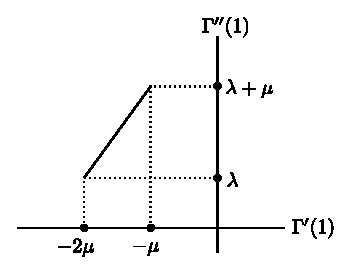
\includegraphics{vol71-figures/fig2.6-1.eps}
\medskip
\caption{}\label{fig2.6.1}
\end{figure}

 Now to choose a convex function $\Gamma : ]0$, $+ \infty [ \to
    \mathbb{R}$ satisfying \eqref{eq2.6-50}. One can find $\alpha \geq 0$,
    $\beta >0$ such that 
  \begin{equation*}
\Gamma (\delta) = \alpha \delta^2 - \beta \log \delta. \tag
    {2.6-55}\label{Eq2.6-55} 
 \end{equation*} 
 
 This function also is such that $\Gamma (\delta) \to + \infty
 ~\text{as}~ \delta \to o^+$.  
 \end{proof}

It follows now that the associated minimization problem has at least
one solution by J.~BALL's theorem. Here 
\begin{multline*}
\mathbb{U}=\{\psi \in \mathbb{H}^1 (\Omega)| \adj (\nabla \psi)
\in \mathbb{L}^2 (\Omega), \det (\nabla \psi) \in L^2 (\Omega),
\det (\nabla \psi)\\
> 0 \text{a.e.}~ \text{and}~ \psi =\phi_0 ~\text{on}~
\Gamma _0 \} \tag{2.6-56}\label{eq2.6-56} 
\end{multline*}
 
\begin{remark}\label{chap2-rem2.6.8} %Remark 2.6.8
In\pageoriginale \eqref{eq2.6-50}, the term $C \delta ^2$ could have been
replaced by $C \delta^ r$, for $r > 1$. The definition fo $\mathbb{U}$
would be modified accordingly.  
\end{remark}

\begin{remark}\label{chap2-rem2.6.9} %Remark2.6.9
It is also possible to choose $\mathcal{X}(F)$ in the form
\begin{equation*}
\mathscr{H}(F)= a_1 \| F \| ^2 +a_2 \| F \|^4 +b \| \adj F \| ^2 +
\Gamma (\det F) \tag{2.6-57}\label{eq2.6-57} 
\end{equation*} 
where $a_1>0, a_2>0, b> 0$ and $\Gamma$ convex. (The St
Venant-Kirchhoff stored energy function resembles this, only
$a_1<0. $). In this case, it can be seen that the admissible range of
values $(\Gamma '(1), \Gamma ''(1))$ lies in the open triangle of
Fig.~\ref{fig2.6.2}. (Exercise 2.6-9).  
\begin{figure}[H]
\centering
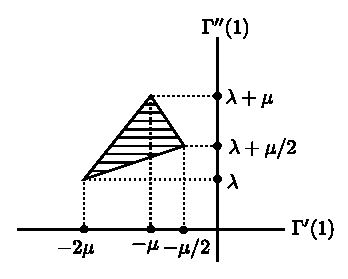
\includegraphics{vol71-figures/fig2.6-2.eps}
\caption{}\label{fig2.6.2}
\end{figure}
\end{remark}

\smallskip
\begin{center}
{\large\bf Exercises}
\end{center}

\begin{description}
\item[2.6-1] Let $\mathscr{H}:\mathbb{M}^3 \to \mathbb{R}$ be a
  function such that 
  $$
  \mathcal{H}(F)= \phi (v_1, v_2, v_3), F \in \mathbb{M}^3_+
  $$
  where $v_i, i=1, 2, 3$ are the principal stretches\index{principal stretch} of $F$. If $\phi$
  is a symetric function which is convex on $(]o, + \infty [)^3$ and
    non-decreasing in each variable, show that $\mathcal{W}$ is
    convex.  

\item[2.6-2] Show\pageoriginale that the stored energy function $\mathcal{W}$
  for a St Venant-Kirchhoff\index{material!St Venant-Kirchhoff}\index{St Venant-Kirchhoff material}  matrial (cf. \eqref{eq2.6-18}) is not
  polyconvex.  

\item[2.6-3] Show that the set
$$
\{\psi \in \mathbb{W}^{1,p}(\Omega)| \adj (\nabla \psi) \in
\mathbb{L}^q (\Omega),q \geq 1 \} 
$$
is not convex $(p \geq 2)$. 

\item[2.6-4] If $p >2$ and $q \leq p/2$ show that $\phi^n
  \rightharpoonup \phi$ in $\mathbb{W}^{1,p}(\Omega)$ implies $\adj
  (\nabla \phi^n)\rightharpoonup \adj (\nabla \phi)$ in
  $\mathbb{L}^q(\Omega)$.  

\item[2.6-5] Show that there exists a constant $d>0$ such that for
  all $\psi \in \mathbb{W}^{1,p}(\Omega), \psi =\psi_0$ on $\Gamma_0$, 
  $$
  \int \limits_\Omega |\psi|^p dx \leq d\left[\int \limits_ \Omega
    |\nabla \psi|^p dx + \left(\int \limits_{\Gamma _o} |\phi_o|
    da\right)^p\right].  
  $$

\item[2.6-6] If $\phi^n \rightharpoonup \phi $ in
  $\mathbb{W}^{1,p}(\Omega)$ and $\phi^n =\phi_o$ on $\Gamma_o$, show
  that $\phi = \phi_o$ on $\Gamma_o$.  

\item[2.6-7] Apply J. BALL's theorem to the mixed
  diaplacement-pressure problem.\index{mixed displacement-pressure problem}

\item[2.6-8]. Let $\tilde{\mathbb{U}}$ be defined by
  \begin{multline*}
  \bar {\mathbb{U}}= \{(\phi ,H) \in \mathbb{H}^1 (\Omega) \times
  \mathbb{L}^2 (\Omega)|H=\adj (\nabla \phi), \phi=\phi_o
  ~\text{on}~ \Gamma_0,\\ 
  \left.\det (\nabla \phi)=1 a. e \right\} 
  \end{multline*}
  (incompressible case).\index{incompressible
  material}\index{material!incompressible} Assume 
  $\tilde{U}= \mathscr{D}$. (i) Show that 
  $\tilde{U}$ is weakly closed in the product space $\mathbb{H}^1
  (\Omega) \times \mathbb{L}^2 (\Omega)$. (ii) Consider 
  \begin{align*}
    \mathcal{W}(F)&= a \| F \|^2 + b \| \adj F \|^2, a>o,b>o,\\
    I(\psi)&= \int \limits _\Omega \mathcal{W}(\nabla \psi)dx-
    (\int \limits _ \Omega f. \psi dx + \int \limits _{\Gamma_1}
    g. \psi da).  
  \end{align*}

  Show that the problem: Find $\phi \in \mathbb{U}$ such that 
{\fontsize{10pt}{12pt}\selectfont
  \begin{multline*}
  \mathbb{U}=\{\phi \in \mathbb{H}^1 (\Omega); \adj  \nabla \phi \in
  \mathbb{L}^2(\Omega), \phi =\phi_o) ~\text{~on~}~ \Gamma_0, \det
  \nabla \phi =1 a . e. \}\\ 
  I(\phi)= \inf_ {\psi \in \mathbb{U}}I (\psi)  
  \end{multline*}\relax}\relax
  has\pageoriginale at least one solution. (iii) If $\phi$ is smooth,
  show that the 
  \textit{Lagrange multiplier} arising out of equality constraint $\det
  (\nabla \phi)=1$, is the pressure.\index{pressure} (cf. Exercise 2.1-2).  

\item[2.6-9.] Check the assertion made in Remark \ref{chap2-rem2.6.9}. 
\end{description}

\newpage

\bigskip
\begin{center}
{\large\bf Bibliography, Comments and some Open Problems}\pageoriginale
\end{center}

\addcontentsline{toc}{chapter}{Bibliography, Comments and some Open Problems}

{\em No attempt} has been made to give an exhaustive list of pertinent
references.  

The first chapter of these lecture notes gave a description of
elasticity in three demensions. For further refrences, one may also
consult GERMAIN [1972], GREEN and ZERNA [1968], GREEN and ADKINS
[1970], GURTIN [1981a, 1981 b], MARSDEN and HUGHES [1978,1983],
STOKER [1968], TRUESDELL and NOLL [1956],\break VALID [1977], WANG and
TRUESDELL [1973], ERINGEN [1962] and WASHING [1975].  

The second chapter discussed some methods for proving the existence of
solution to the boundary value problem of non-linear elasticity and to
the associated variational problem, in the case of hyperelastic
materials.  

For references about the linearized system of elasticity, see DUVAUT
and LIONS [1972], FICHERA [1972] and GURTIN [1972].  

The key result in proving existence via the \textit{implicit function
  theorem} is the $W^{2,p}(\Omega)$-regularity of the linearized
system of elasticity. The case $p=2$ was proved by NECAS [1967] and
the regularity for other $p$ was proved by GEYMONAT [1965]. From
this regularity result, (proved however only for the pure
\textit{displacement problem}) the existence theorem was independently
proved by CIARLET and DESTUYNDER [1979b], MARSDEN and HUGHES
[1978], VALENT [1979]. The basic idea, however, goes back to
SPOPPELLI [1954] and VAN BUREN [1968]. The extension of this result
to more general constutive equations was particularly studied by
VALENT [1979]. See also VALENT [1978a, 1978b].  

The\pageoriginale necessity of the $W^{2,p}(\Omega)$-regularity of the
linearized 
problem restricts the application of this method to \textit{pure
  displacement problems.} It is also possible to treat the \textit{pure
  traction problem,} which is more complicated owing to the
compability conditions which the given forces must satisfy. For
details see CHILLINGWORTH, MARSDEN and WAN [1982].  

The increment method described in Section \ref{chap2-sec2.4} is none
other than Euler's method for approximating an appropriate
differential equation in a Solbolev space. In other words, this method
appears as an 
infinite demensional version of the so called \textit{continuation by
  differentiation} approach as described, for instance, in RHEINBOLDT
[1974].  

To the best of the author's Knowledge, the convergence of increment
methods for non-linear elasticity problems has been analysed so far
only in some special cases, such as the one demensional model of a
thin shallow spherical shell, by ANSELONE and MOORE [1966] or some
finite dimensional structural problems by RHEINBOLDT [1981]. The
results presented in these lecture can be found in BERNADOU, CIARLET
and HU [1982].  

For a decription of incremental methods in non-linear elasticity see
MASON [1980], ODEN [1972] and WASHIZU [1975].  

The variation approach is based on the famous article of BALL
[$1977$]. In addition to the notion of \textit{polycomvexity} another
essential contribution of J. BALL is that one can pass to the weak
limit in certain non-convex sets as was seen in Section 2.6. This
idea of compactness by compensation was also developed by MURAT
[1978, 1979] and TARTAR [1979]. See also AUBERT and TAHRAOUI
[1982].  

Other\pageoriginale important refrences are BALL [1981a,1981b, 1981c], BALL,
CURRIE and OLIVER [1981], BALL, KNOPS and MARSDEN [1978]. See also
EKELAND and TEMAN [1974] for the general problem of minimizing
functionals.  

The notion of polyconvexity led to the definition of an {\em Ogden's
material} (cf. OGDEN [1972]). A \textit{St Venant-Kirchhoff
  material} is not Ogden's material and the existence of a solution to
the corresponding mixed displacement-traction problem is open. In this
connection see also ATTEIA and DEDIEU [1981] and DACOROGNA [1982a,
  1982b]. For yet another approach, see ODEN [1979].  

One of the drawbacks of J. BALL's approach is the lack of regularity
of the solution and so one does not know if the solution thus obtained
satisfies the \textit{equilibrium equation} even in a weak sense. In
this contex, see the results of LE TALLEC [1981] and LE TALLEC and
ODEN [1981] for incompressible materials.  

To conclude, we present a list of some of the open problems in
non-linear elasticity. Some of them have been mentioned in the text
before.  

\begin{enumerate}[1.]
\item Let $C=\nabla \phi^T \nabla \phi$. If $C-I$ is
  'small', in a sense to be made precise, can it be said that $\phi$
  is close to a rigid deformation? If some boundary conditions are
  imposed, can it be shown that $\phi$ is one-one? 

In this context cf. KOHN [1982], ALEXANDER and ANTHAN [1982],
ANTMAN [1979].  

\item The\pageoriginale standard implicit function theorem approach
  fails for mixed\break 
  problems. Could ``hard" implicit function theorem like that of NASH
  and MOSER be used? In case of special domains like a thin plate,
  the singularities are know explicity. Could this be used, and the
  implicit function theorem used only on the ``regular" part of the
  solution? 
\item Study of incremental methods taking into account the finite
  element methods.  
\item An incremental method can be \textit{formally} written down for
  the mixed problem. If it can be shown to be convergent, this would
  provide an existence theorem for the mixed problem.  
\item The minimization procedure of J BALL does not imply that the
  solution is small if the forces are small. How can one
  ``distinguish" the expected small solution in this case? (In the
  case of the pure displacement problem, the solution via the implicit
  function theorem does not seem to be a local minimum of the energy
  in the ``right" space).  
\item A study \textit{plasticity} has been taken up by TEMAN and
  STRANG\-[1980a, 1980b]. They use the linear theory in the part
  corresponding to elasticity. Can one obtain better results by
  incorporating the non-linear theory, using J. BALL's approach? 
\item A study of `non local' constotutive equations. Here the
  comstitutive equation is of the form 
$$
T(x)= \int \limits_{\mathbb{B}} \rho_k (x-y) \hat{T} (\nabla \phi (y))dy
$$
where $\rho_k$ is a \textit{mollifier.}

\item One\pageoriginale of the \textit{hardest} open problems of the
study of the 
  \textit{evolution problem} which is a non-linear hyperbolic
  problem. The only available results are in the one-demensional case
  due to DIPERNA [1983]. See also HUGHES, KATO and MARSDEN [1976].  
\item Plate theory. A plate can be thought of as a domain $\Omega^\in
  = \omega \times ]-\in,+ \in [$, where $\omega \subset \mathbb{R}^2$
    is a bounded open set and $\in >o$ is a small
    parameter. (cf. Fig.1) 
    
    \begin{figure}[H]
      \centerline{
        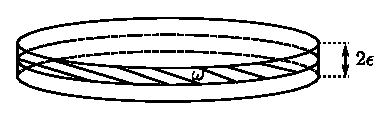
\includegraphics{vol71-figures/fig1.eps}}
      \medskip
      \centerline{\bf Figure~1}
    \end{figure}

    By methods of asymptotic expansions, the solution $(u^\in, \sigma
    ^\in)$ can be formally expanded as 
    $$
    (u^\in, \sigma^\in)=(u^0, \sigma^0)+(u^1, \sigma^1)+ \cdots
    $$
where $(u^0, \sigma ^0)$ satisfies a well-known two-dimensional plate
model. In the linearized theory CIARLET and DESTUYNDER [1980a],\break
CIARLET and KESAVAN [1980], DESTUYNDER [1980] have stu\-died the
problems extensively. One can compare the three dimensional and two
dimensional problems and show that (for example) 
$$
\frac {\| u^ \in_{3d}-u^\in _{2d} \| _{1,\Omega^\in}} {\| u^\in _{3d}
  \| _{1 ,\Omega ^\in}} \to o ~\text{as}~ \in \to 0.  
$$ 

The problem is to \textit{numerically} verify this. Computing by the
finite element method, one gets $ u^ \in_{3d,h}$ and $ u^ \in_{2d,h}$
approximating $ u^ \in_{3d}$ and $u^ \in_{2d}$ respectively. Since
$\in$ is small, unless $h$ is of the same order, 
 the\pageoriginale linear systems become very ill-conditioned. But if $h$ is of the
 same order of $\epsilon$, the solution $u^{\epsilon}_{3d,h}$ is
 not very accurate. Thus to find a better method of approximating
 these solutions and verify the convergence described above. 

 \item In the nonlinear case CIARLET [1980] (see also CIARLET and\-
   DESTUYNDER [1979], CIARLET and RABIER [1980]) has shown that
   with certain boundary conditions the three dimensional plate model
   for a St Venant -Kirchhoff material is approximated (formally) by
   the well-known two-dimensional von Karman model. While the latter
   has a satisfactory existence theorey, the former has none. If at
   least for $\epsilon$ small enough it can be shown that the three
   dimensional problem has a solution converging to a given solution
   of the dimensional problem, an existance theorem for such special
   domains can be obtained. 
 \end{enumerate}


\begin{thebibliography}{99}\pageoriginale
\bibitem{1}{ADAMS, R.A. (1975):} Sobolev Spaces, academic Press, New York.
\bibitem{2}{AGMON, S., DOUGLIS,A. and NIRENBERG,L.(1959):} Estimates
  near the boundary for solutions of elliptic partial defferential
  equations satisfying general boundary conditions $I$. Comm. Pure
  Appl. Math., 12,pp.623-727. 
\bibitem{3}{AGMON, S.,DOUGLIS,A. and NIRENBERG,L.(1964):} Estimates
  near the boundary for solutions of elliptic partial defferential
  equations satisfying general boundary conditions $II$, Comm. Pure
  Appl. Math., 17,pp.35-92. 
\bibitem{4}{ALEXANDER, J.C. and ANTMAN,S.S. (1982):} The ambiguous
  twist of Love, Quart. Appl. Maths., pp.83-92. 
\bibitem{5}{ANSELONE,P.M. and MOORE (1966):} An extension of the
  Newton Kantorovic method for solving nonlinear equation with an
  application to elasticity, J.Math.Anal. Appl., 13.pp. 476-501. 
\bibitem{6}{ANTAM, S.S.(1979):} The eversion of thick spherical
  shells, Arch. Rational Mech . Anal., 70,pp.113-123. 
\bibitem{7}{ATTEIA,M. and DEDIEU,J.P.(1981):} Minimization of energy
  in non linear elasticity, in Nonlinear Problems of analysis in
  Geometry and Mechanics, [M.ATTEIA, D. BANCEL, I. GUMOWSKI, Editors],
  pp.73-79, Pitman, Boston 
\bibitem{8}{AUBERT,G.and TAHRAOUI,R.(1982):} Sur la faible fermeture
  de certain ensembles de contraintes en elasticite non-lineaire
  plane, Arch. Rational Mech. Anal, to appear. 
\bibitem{9}{BALL,J.M. (1977):}\pageoriginale Convexity conditions and existance
  theorems in nonlinear elasticity, arch. Rational. Mech. Anal.,
  63,pp.337-403. 
\bibitem{10}{BALL,J.M.(1981a):} Discontinuous equilibrium solutions
  and cavitions in non-linear elasticity, Phil. Trans. Rayal
  Soc. London, to appear. 
\bibitem{11}{BALL,J.M. (1981b):} Remarques sur $\ell'$ existance et la
  regularite des solutions d'\'elastostatique non-lineare, in Recent
  Contributins to Nonlinear Partial Differential Equations,
  pp.50-62, Res. Notes in Math., 50, Pitman, Boston. 
\bibitem{12}{BALL,J.M. (1981c):} Global invertibility of 'Sobolev
  functions and the interpenetration of matter,Proc. Royal
  Soc. Edinburgh, 88A, pp.315-328. 
\bibitem{13}{BALL,J.M., CURRIE,J.C. and OLVER,P.J.(1981):} Null
  Lagrangians, weak continuit and variational problems of arbitrary
  order, J.Functional analysis, 41, pp.135-174.  
\bibitem{14}{BALL,J.M., KNOPS,R.J. and MARSDEN,J.E. (1978):} Two
  examples in non-linear elasticity, in Proceedings, conference on
  nonlinear Analysis, Besancon, 1977, pp.41-49, Springs-Verlag,
  Berlin. 
\bibitem{15}{BERNADOU,M., CIARLET, P.G. and HU,J. (1982):} Sur la
  convergence des m\'ethodes incr\'ementales en \'elasticite non-lin\'eare
  tridimensionnelle. C.R.Acad, Sc. Paris, S\'erie I, 295. 639-642.  
\bibitem{16}{CHILLINGWORTH,D.R.J.,MARSDEN, J.E.and WAN, Y.H. (1982):}
  Symmetry and bifurcation in three dimensional elasticity. Part
  $I$., Arch. Rational Mech, Anal., 80, pp.295-331. 
\bibitem{17}{CIARLET,P.G. (1980):} A justification of the von Karman
  equations, Arch. Rational Mech.Anal., 73, pp.349-389. 
\bibitem{18}{CIARLET,\pageoriginale P.G. and DESTUYNDER,P.(1979a):} A
justification 
  of the two-dimensional linear plate model, J.Mecanique,
  18, pp.315-344. 
\bibitem{19}{CIARLET,P.G. and DESTUYNDER,P.(1979b):} A justification
  of a nonlinear model in plate theory, Compute. Methods
  Appl. Mech. Engrg., 17/18, pp.227-258.  
\bibitem{20}{CIARLET,P.G. and GEYMONAT,G.(1982):} Sur les lois de
  comportment en elasticite non-lineaire compressible,
  C.R. Acad. Sci. Paris, Serie A., 295,pp.423-426. 
\bibitem{21}{CIARLET,P.G. and KESAVAN,S.(1980):} Tow dimensional
  approximations of three-dimensional eigenvalues in plate theory,
  Compute. Methods Appl. Mech. Engrg., 26, pp.149-172.  
\bibitem{22}{CIARLET, P.G. and RABIER, P. (1980):} Les Equations de
  von Karman, Lecture notes in Mathematics, Vol. 826,
  Springer-Verlag,Berlin.  
\bibitem{23}{DACOROGNA,B.(1980a):} Weak Continuity and Weak Lower
  Semicontinuity of Non-Linear Functionals. Lecture Notes in
  Mathematics, Vol.922, Springer-Verlag, Berlin. 
\bibitem{24}{DACOROGNA,B. (1982b):} Quasiconvexity and relaxation of
  non-convex problems in the calculus of variations, j. Functional
  Analysis 46, pp.102-118. 
\bibitem{25}{DESTUYNDER,P. (1980):} Sur une Justification dea Modeles
  de plaques et de Coques par les Methodes Asymptotiques,
  Thesis,univesite Pierre et Marie Curie, Paris. 
\bibitem{26}{DESTUYNDER,P. and GALBE,G.(1978):} Analyticite de la
  solution $d'$ un probleme hyperelastique nonlineare,
  C.R. Acad. Sci. Paris, Serie A, pp.365-368. 
\bibitem{27}{DIPERNA,\pageoriginale R.J.(1983):} To appear
\bibitem{28}{DUVAUT,G. and LIONS,J.L.(1972):} Les Inequations en
  Mecanique et en Physique, Dunod, Paris. 
\bibitem{29}{EKELAND, I, and TEMAM,R.(1974):} Analyse Convexe et
  Problems Variationnels, Dunod, PAris. (English Translation: Convex
  Analysis and Variational Problems, North Holland, Amsterdam, 1975). 
\bibitem{30}{ERINGEN,A.C. (1962):} Nonlinear Theoey of Continuous
  Media, McGraw-Hill, New York. 
\bibitem{31}{FICHERA,G.(1972):} Existence theorems in elasticity,
  Handbuch der Physik, VIa/2, Springer, Berlin. 
\bibitem{32}{GERMAIN,P.(1972):} Mecanique des Milieux Continuous, Tome
  1 Massan, Paris.  
\bibitem{33}{GEYMONAT,G.(1965):} Sui problems ai limiti per $i$
  sistemi lineari ellitici, Ann. Mat. Pura. Appl., 69, pp.207-284. 
\bibitem{34}{GREEN,A.E. and ADKINS, J.E. (1970):} Large Elastic
  Deformations, Second Edition, Clarendon Press, Oxford. 
\bibitem{35}{GREEN,A.E. and ZERNA, W.(1968):} Theoretical Elasticity,
  university Press, Oxford. 
\bibitem{36}{GURTIN, m.E. (1972):} The linear theory of elasticity, in
  Handbuch der Physik, pp.1-295, Vol. VIa, Springer-Verlag,
  Berlin. 
\bibitem{37}{GURTIN,M.E.(1981a):} Topics in Finite Elasticity,
  CBMS-NSF Regional Conference Series in Applied Mathematics, SIAM,
  Philadephia. 
\bibitem{38}{GURTIN,M.E. (1981b):} Introduction to Continuous
  Mechanics, Academic Press, New York. 
\bibitem{39}{HUGHES,\pageoriginale T.J.R., KATO, T, and MARSDEN,J.E.(1976):}
  Well-posed quasi linear second -order hyperbolic system with
  applications to non-linear elastodynamics and general relativity,
  Arch. Rational Mech. Anal., 63, pp. 273-304. 
\bibitem{40}{JOHN,F.(1972):} Uniqueness of non-linear elastic
  equilibrium for prescrbed boundary displacements and sufficiently
  small strains, Comm. Pure Appl. Math., XXV, pp.617-634. 
\bibitem{41}{KOHN, R.V. (1982):} New integral estimates for
  deformations in terms of their nonlinear, Arch. Rational Mech,
  Anal., 78, pp. 131-172. 
\bibitem{42}{LE DRET,H. (1982):} Thesis, Universite Pierre et MArie
  Curie, Paris. 
\bibitem{43}{LE TALLEC,P. (1981):} Existence and approximation results
  for non-linear mixed problems: applications to incompressible finite
  elasticity, (to appear). 
\bibitem{44}{LE TALLEC, P. and ODEN,J.T. (1981):} Existence and
  characterization of hydrostatic pressure in finite deformations of
  incompressible elastic bodies, J. Elasticity, 11, pp.341-358. 
\bibitem{45}{MARSDEN,J.E. and HUGHES, T.J.R. (1978):} Topics in the
  mathematical foundations of elasticity, in Nonlinear Analysis and
  Mechanics: Heriot-Watt Symposim, Vol.2, pp.30-285, Pitman,
  London.  
\bibitem{46}{MARSDEN,J.E. and HUGHES, T.J.R. (1983):} Mathematical
  Foundations of Elasticity, Prentice-Hall, Englewood Cliffs. 
\bibitem{47}{MASON,J. (1980):} Variational, Incremental and Energy
  Methods in Solid Mechanics and Shell Theory, Elsevier, Amsterdam.  
\bibitem{48}{MEISTERS,G.H. and OLECH, C. (1963):} Locally one-to -one
  mapping and a classical theorem on Schlicht functions, Duke
  Math. J., 30, pp.63-80. 
\bibitem{49}{MURAT,\pageoriginale F. (1978):} Compacite par compesation,Annali
  Scu. Norm. Sup. Pisa. IV, 5, pp. 489-507. 
\bibitem{50}{MURAT,F.(1979):} Compacite par compensation
  II. Proceedings International Conference on recent Methods in-Linear
  Analysis, Rome, 1978, Pitagora, Bologna, 
\bibitem{51}{NECAS,J.(1967):} Les Methodes Directes en Theorie des
  Equations Elliptiques, Masson, Paris. 
\bibitem{52}{NITSCHE,J.A. (1981):} On Korn's Second inequality, RAIRO,
  Analyse Numerique, Vol.15, No.3, pp. 237-248. 
\bibitem{53}{ODEN,J.T. (1972):} Finite Elements of Nonliner Continua,
  McGraw-Hill New York. 
\bibitem{54}{ODEN,J.T.(1979):} Existance theorems for a class of
  problems in non-linear elasticity, J. Math.Anal. Appl., 69, pp.51-83.  
\bibitem{55}{OGDEN, R.W. (1972):} Large deformation isotrophic
  elasticity: On the correlation of theory and experiment for
  compressible rubberlike solids, proc. Roy. Soc. London, A
  328, pp.567-583.  
\bibitem{56}{RHEINBOLDT,W.C. (1974):} Methods for Solving Systems of
  Nonlinear Equations, CBMS Series, No.14, SIAM, Philadephia. 
\bibitem{57}{RHEINBOLDT,W.C. (1981):} Numerical analysis of
  continuation methods for nonlinear structure problems, Computers and
  structures, 13, pp.103-113. 
\bibitem{58}{STOKER,J.J.(1968):} Nonlinear Elasticity, Gordon and
  Breach, New York. 
\bibitem{59}{STOPPELLI,F.(1954):} Un teorema di esistenza e ~di
  unicita relativo alle equazioni dell' elastostatica isoterma per
  deformazioni finite, Ricerche di Matematica, 3, pp.247-267. 
\bibitem{60}{TARTAR,\pageoriginale L. (1979):} Compensated compactness and partial
  differential equation, in Nonlinear Analysis Mechanics: Heriot-Watt
  Symposim, Vol. IV,(R.J.knops, Ed.) Pitman, pp.136-212. 
\bibitem{61}{TEMAM,R. and STRANG,G. (1980a):} Duality and relaxation
  in plasticity, J. de Mecanique, 19, pp.1-35.  
\bibitem{62}{TEMAM, R. and STRANG, G.(1980b):} Functions of bounded
  deformation Arch. Rational Mech.Anal., 75, pp.7-21. 
\bibitem{63}{TRUESDELL,C. and NOLL,W. (1965):} The Non-linear field
  theories of Mechanics. Handbuch der Physik, Vol.III/3, Springer,
  Berlin. 
\bibitem{64}{VALENT,T. (1978a):} Sulla Defferenziabilita di un
  operatore legato a una classe di sistemi differenziali
  quasi-lineari, Rend. Sem. Mat. Univ. Padova, 57,pp.311-322. 
\bibitem{65}{VALENT,T. (1978b):} Osservazioni sulla linearizzazione di
  un operatore differenziale, Rend. Acc. Naz. Lincei, 65,pp.27-37.
\bibitem{66}{VALENT, T. (1979):} Teoremi di esistenza e unicita in
  elastostatica finite, Rend. Sem. Mat. univ. Padova, 60, pp.165-181. 
\bibitem{67}{VALID,R. (1977):} La Mecanique des Milieux Continus et le
  Coloul des Structures. Eyrolles, Paris. (English translation:
  Mechanics of Continuous Media and Analysis of Stuctures
  North-Holland, Amsterdam, 1981). 
\bibitem{68}{VAN BUREN, M. (1968):} On the Existence and Uniqueness of
  Solutions to Boundary Value Problems in Finite Elasticity, Thesis,
  Carnegie-Mellon University. 
\bibitem{69}{WANG, C,-C. and TRUESDELL,C.(1973):} Introduction to
  Rational Elasticity, Noordhoff, Groningen. 
\bibitem{70}{WASHIZU, K.(1975):} Variational Methods in Elasticity and
  Plasticity, Second Edition, Pergamon, Oxford.  
 \end{thebibliography} 

\newpage



\begin{center}
{\Large\bf List of Notations}\pageoriginale
\end{center}

\addcontentsline{toc}{chapter}{List of Notations}

\noindent
{\bf General Conventions:} (1) Unless otherwise indicated, Latin indices
take their values in the set $\{1,2,3\}$, and the repeated index
convention for summation is systematically used in conjunction with
this rule.

(2)~ If a quantity is denoted $X$ in the deformed configuration, the
corresponding quantity in the reference configuration is denoted
$X_{R}$.

\bigskip
\noindent
{\bf Vectors and Matrices}
\begin{longtable}{@{}>{$}r<{$}@{\;}c@{\;}p{6.7cm}<{\raggedright}@{}}
(e_{i}) & : & orthonormal basis in $\mathbb{R}^{3}$\\
v=(v_{i}) & : & vector $v$ with components $v_{i}$\\
A=(A_{ij}) & : & matrix $A$ with elements $A_{ij}$ ($i:$ row index,
$j:$ column index)\\
u\cdot v=u_{i}v_{i} & : & Euclidean inner product\\
|u|=\sqrt{u\cdot u} & : & Euclidean vector norm\\
\mathscr{E}_{ijk} & = & $\begin{cases} +1\text{\ if\ } (i,j,k)\text{ \
is an even permutation of\ }\\ 
\hfill (1,2,3)\\
-1\text{\ if\ } (i,j,k) \text{\ is an odd permutation of\ }\\
\hfill (1,2,3)\\
0\text{\  otherwise}
\end{cases}$\\
u\Lambda v=\mathscr{E}_{ijk}u_{j}b_{k}e_{i} & : & cross product in
$\mathbb{R}^{3}$\\
A:B=A_{ij}B_{ij}=\tr(AB^{T}) &:& matrix inner product\\
||A||=\sqrt{A:A} &:& matrix norm associated with the matrix inner
product\\
A^{-T} &:& $(A^{-1})^{T}$ ($A^{-1}$: inverse matrix;\\
 &&\quad $A^{T}$: transposed matrix).\\
adj $A$ &:& adjugate of a matrix (transpose of the cofactor matrix)\\
l_{A}=(l_{1}(A);l_{2}(A),l_{3}(A)) &:& set of the principal
invariants of a matrix of order 3\\
l_{1}(A) &=& $a_{ii}=\tr(A)$\\
l_{2}(A) &=& $\frac{1}{2}(a_{ii}a_{jj}-a_{ij}a_{ij})(=\det A\tr
A^{-1}$ if $A$ is invertible)\\
l_{3}(A) &=& $\det A$\\
\mathbb{M}^{3} &:& set of all matrices of order 3\\
\mathbb{M}^{3}_{+} &=& $\{F\in\mathbb{M}^{3}|\det F>0\}$\\
\mathbb{O}^{3} &=& $\{F\in\mathbb{M}^{3}|F^{T}F=FF^{T}=I\}$\\
\mathbb{O}^{3}_{+} &=& $\mathbb{O}^{3}\cap
M^{3}_{+}=\{F\in\mathbb{O}^{3}|\det F=1\}$\\
\mathbb{S}^{3} &=& $\{F\in\mathbb{M}^{3}|F=F^{T}\}$\\
\mathbb{S}^{3}_{>} &=& $\{F\in\mathbb{S}^{3}|F\text{ is positive
definite}\}$\\ 
F=RU &=& $VR:$ polar factorization of an invertible matrix
$(R\in\mathbb{O}^{3};U,V\in\mathbb{S}^{3}_{>})$\\ 
C^{1/2} &:& square root of a matrix $C\in\mathbb{S}^{3}_{>}$
\end{longtable}\pageoriginale

\medskip
\noindent
{\bf Functions and Function Spaces}
\begin{longtable}{@{}>{$}r<{$}@{\;}c@{\;}p{6.5cm}<{\raggedright}@{}}
\Id &:& identity mapping\\
v'(a) &:& Fr\'echet derivative of the mapping $v$ at the point $a$\\
\partial^{\alpha}v &=& $\dfrac{\partial^{|\alpha|}v}{\partial
x^{\alpha_{1}}_{1}\ldots \partial x^{\alpha_{n}}_{n}}$,
$|\alpha|=\alpha_{1}+\cdots+\alpha_{n}$ (multi-index notation for
partial derivatives)\\
\dfrac{\partial\mathscr{W}}{\partial F}(F) &=&
$\left(\dfrac{\partial\mathscr{W}}{\partial
F_{ij}}(F)\right)\in\mathbb{M}^{3}$ (for a mapping
$\mathscr{W}:\mathbb{M}^{3}\to \mathbb{R}$)\\
X\hookrightarrow Y &:& the canonical injection from $X$ into $Y$ is
continuous\\ 
X\displaystyle{\mathop{\hookrightarrow}^{c}}Y &:& the canonical
injection from $X$ into $Y$ is compact\\
\rightharpoonup &:& weak convergence\\
C^{0}(X,Y) &:& set of all continuous mappings from $X$ into $Y$\\
C^{m}(X;Y) &:& space of all $m$ times continuously differentiable
mappings from $X$ into $Y(1\leq m\leq \infty)$\\
C^{m}(X) &=& $C^{m}(X;\mathbb{R})$, $0\leq m\leq \infty$.\\
W^{m,p}(\Omega) &=& $\{v\in L^{p}(\Omega);\partial^{\alpha}v\in
L^{p}(\Omega)$ for all $|\alpha|\leq m\}$
$(W^{0,p}(\Omega)=L^{p}(\Omega))$\\
H^{m}(\Omega) &=& $W^{m,2}(\Omega)$\\
\mathbb{L}^{p}(\Omega),\mathbb{W}^{m,p}(\Omega),\mathbb{H}^{m}(\Omega)
&:& corresponding spaces of vector-valued, or matrix-valued,
functions\\
|v|_{0,p,\Omega} &:& norm of the space $L^{p}(\Omega)$, $1\leq
p\leq \infty$.\\
||v||_{m,p,\Omega} &=&
$\{\int\limits_{\Omega}\sum\limits_{|\alpha|\leq
m}|\partial^{\alpha}v|^{p}dx\}^{1/p}$: norm of the space
$W^{m,p}(\Omega)$, $1\leq p\leq \infty$\\
||v||_{m,\infty,\Omega} &=& $\max\limits_{|\alpha|\leq
m}|\partial^{\alpha}v|_{0,\infty,\Omega}$: norm of the space
$W^{m,\infty}(\Omega)$\\ 
|v|_{m,p,\Omega} &=&
$\{\int\limits_{\Omega}\sum\limits_{|\alpha|=m}|\partial^{\alpha}v|^{p}dx\}^{1/p}$,
$1\leq p\leq \infty$\\
|v|_{m,\infty,\Omega} &=&
$\max\limits_{|\alpha|=m}|\partial^{\alpha}v|_{0,\infty,\Omega}$\\ 
\mathscr{D}(\Omega) &=& $\{v\in\mathscr{C}^{\infty}(\Omega);\supp v$
is a compact subset of $\Omega\}$\\
W^{m,p}_{0}(\Omega) &:& closure of $\mathscr{D}(\Omega)$ in
$W^{m,p}(\Omega)$\\
H^{m}_{0}(\Omega) &=& $W^{m,2}_{0}(\Omega)$
\end{longtable}\pageoriginale

\medskip
\noindent
{\bf Miscellaneous}
\begin{longtable}{@{}>{$}r<{$}@{\;}c@{\;}p{6.5cm}<{\raggedright}@{}}
[a,+\infty] &=& $[a,+\infty[\cup \{+\infty\},a\in R$\\
f(x) =0(x) &:& $\lim\limits_{\substack{x\to 0\\ x\neq
0}}\dfrac{|f(x)|}{||x||}=0$\\
c\circ U &:& convex hull of $U$ (smallest convex set containing $U$)
\end{longtable}

\medskip
\noindent
{\bf Notations in the Deformed Configuration}\pageoriginale
\begin{longtable}{@{}>{$}r<{$}@{\;}c@{\;}p{6.5cm}<{\raggedright}@{}}
\mathscr{B}=\phi(\mathscr{B}_{R}) &:& deformed configuration\\
X=\phi(X_{R}) &:& generic point of $\mathscr{B}$\\
\partial \mathscr{B} &:& boundary of $\mathscr{B}$\\
\partial \mathscr{B}=\partial \mathscr{B}_{0}\cup \partial \mathscr{B}_{1}
&:& $dA$-measurable partition of $\partial \mathscr{B}$\\
n &:& unit outer normal along $\partial \mathscr{B}$\\
dX &:& volume element in $\mathscr{B}$\\
dA &:& surface element on $\partial \mathscr{B}$\\
\text{GRAD\,}\Theta &=& $\left(\dfrac{\partial \Theta_{i}}{\partial
X_{j}}\right)\in \mathbb{M}^{3}$ (for a mapping
$\Theta:\mathscr{B}\to \mathbb{R}^{3}$)\\ 
\text{DIV~T}=\dfrac{\partial T_{ij}}{\partial
X_{j}}e_{i}\in\mathscr{R}^{3} &:& divergence of a tensor field
$T:\mathscr{B}\to \mathbb{M}^{3}$\\
\partial (X)\in\mathbb{R} &:& density per unit mass at
$X\in\mathscr{B}$\\
b(X)\in\mathbb{R}^{3} &:& body force density per unit mass at
$X\in\mathscr{B}$\\ 
t_{1}(X)\in\mathbb{R}^{3} &:& applied surface force density per unit
area of $\partial \mathscr{B}$ at $X\in\partial\mathscr{B}$\\
t(X,n),X\in\mathscr{B},|n|=1 &:& Cauchy stress vector in
$\mathscr{B}$\\
T(X) &:& Cauchy stress tensor at $X\in\mathscr{B}$\\
\hat{T},\overline{T} &:& response function for
$T=\hat{T}(F)=\overline{T}(B)$, with $F\in\mathbb{M}^{3}_{+}$, $B=FF^{T}$.
\end{longtable}

\medskip
\noindent
{\bf Notations in the Reference Configuration}\pageoriginale
\begin{longtable}{@{}>{$}r<{$}@{\;}c@{\;}p{4.5cm}<{\raggedright}@{}}
\mathscr{B}_{R},\text{ or } \overline{\Omega} &:& reference
configuration\\
X_{R},\text{ or } x &:& generic point of $\mathscr{B}_{R}$\\
\partial \mathscr{B}_{R}, \text{ or } \Gamma &:& boundary of
$\mathscr{B}_{R}$\\
\partial\mathscr{B}_{R}=\partial \mathscr{B}_{0R}\cup \partial \mathscr{B}_{1R},\text{
or } \Gamma = \Gamma_{0}\cup \Gamma_{1} &:& $dA_{R}$-measurable
partition of $\partial \mathscr{B}_{R}$\\
n_{R}, \text{ or }\nu &:& unit outer normal along
$\partial \mathscr{B}_{R}$\\
dX_{R},\text{ or } dx &:& volume element in $\mathscr{B}_{R}$\\
dA_{R},\text{ or } da &:& surface element on
$\partial \mathscr{B}_{R}$\\
\phi,\psi:\mathscr{B}_{R}\to \mathbb{R}^{3} &:& deformation of
$\mathscr{B}_{R}$ (smooth maps with $\det\cdot >0$)\\
u, v:\mathscr{B}_{R}\to \mathbb{R}^{3} &:& displacement
$(\phi=\Id+u,\psi=\Id+v)$\\
\partial_{i} &=& $\dfrac{\partial}{\partial X_{R_{i}}}$\\
\text{DIV}_{R}T_{R}=\frac{\partial T_{Rij}}{\partial
X_{R_{j}}}e_{i}\in\mathbb{R}^{3} &:& divergence of a tensor field
$T_{R}:\mathscr{B}_{R}\to \mathbb{M}^{3}$\\
\nabla_{\phi} =\left(\frac{\partial \phi_{i}}{\partial
X_{R_{j}}}\right)\in\mathbb{M}^{3}_{+} &:& deformation gradient\\
\nabla_{u}=\left(\frac{\partial u_{i}}{\partial
X_{R_{j}}}\right)\in\mathbb{M}^{3} &:& displacement gradient\\
C=\nabla_{\phi}^{T}\nabla_{\phi}\in\mathbb{S}^{3}_{>} &:& right
Cauchy-Green strain tensor\\
B=\nabla_{\phi}\nabla_{\phi}^{T}\in\mathbb{S}^{3}_{>} &:& left
Cauchy-Green strain tensor\\
E=E(u)=\frac{1}{2}(C-I) &=& $\dfrac{1}{2}(\nabla u^{T}+\nabla u+\nabla
u^{T}\nabla u)$: Green-St Venant strain tensor\\
\epsilon(u)=\dfrac{1}{2}(\nabla u^{T}+\nabla u) &:& linearized strain
tensor\\
\rho_{R}(X_{R})\in\mathbb{R} &:& density per unit mass at
$X_{R}\in\mathscr{B}_{R}$\\ 
b_{R}(X_{R})\in\mathbb{R}^{3} &:& body force density per unit mass at
$X_{R}\in\mathscr{B}_{R}$\\ 
f &=& $\rho_{R}b_{R}:\Omega\to \mathbb{R}^{3}$\\
t_{1R}(X_{R})\in\mathbb{R}^{3} &:& applied surface force density per
unit area of $\partial \mathscr{B}_{R}$ at
$X_{R}\in\partial\mathscr{B}_{R}$\\ 
g &=& $t_{1R}:\Gamma_{1}\to \mathbb{R}^{3}$\\
t_{R}(X_{R},n_{R}),X_{R}\in\mathscr{B}_{R},|n_{R}|=1 &:& first
Piola-Kirchhoff stress vector in $\mathscr{B}_{R}$\\
T_{R}(X_{R}) &:& first Piola-Kirchhoff stress tensor at
$X_{R}\in\mathscr{B}_{R}$\\
(t_{ij})=T_{R} &:& $\Omega\to \mathbb{M}^{3}$\\
\hat{T}_{R} &:& response functions for $T_{R}=\hat{T}_{R}(F)$,
$F\in\mathbb{M}^{3}_{+}$\\ 
\sum_{R}(X_{R})=\nabla_{\phi}(X_{R})^{-1}T_{R}(X_{R}) &:& second
Piola-Kirchhoff stress tensor at $X_{R}\in\mathscr{B}_{R}$\\
(\sigma_{ij})=\sum_{R} &:& $\Omega\to \mathbb{S}^{3}$\\
\hat{\sum}_{R},\overline{\sum}_{R},\sum^{\ast}_{R} &:& response
functions for
$\sum_{R}=\hat{\sum}_{R}(F)=\overline{\sum}_{R}(C)=\sum^{\ast}_{R}(E)$,
with $F\in \mathbb{M}^{3}_{+}$, $C=F^{T}F=I+2E$\\
\sigma^{\ast}(E) &:& $\sum^{\ast}_{R}(E)=\lambda(\tr E)I+2\mu
E+0(E)$\\
\lambda,\mu &:& Lam\'e's constants\\
\nu=\dfrac{\lambda}{2(\lambda+\mu)} &:& Poisson's ratio\\
E=\dfrac{\mu(3\lambda+2\mu)}{\lambda+\mu} &:& Young's modulus\\
a_{ijk\ell}=\lambda\delta_{ij}\delta_{k\ell}+2\mu\delta_{ik}\delta_{j\ell}
&:& elasticity coefficients for isotropic materials\\
\mathscr{W} &:& stored energy function
$\left(\dfrac{\partial \mathscr{W}}{\partial
F}(R)=\hat{T}_{R}(F),F\in\mathbb{M}^{3}_{+}\right)$\\ 
\overline{\mathscr{W}} &:& stored energy function in terms of
$C=F^{T}F(\mathscr{W}(F)=\overline{\mathscr{W}}(C))$\\ 
\mathscr{W}^{\ast} &:& stored energy function in terms of
$E(\mathscr{W}(F)=\overline{\mathscr{W}}(I+2E)=\mathscr{W}^{\ast}(E))$\\
\phi &:& stored energy function in terms of
$l_{c}:\mathscr{W}(F)=\phi(l_{c}),C=F^{T}F$\\ 
W(\psi)=\int\limits_{\mathscr{B}_{R}}\mathscr{W}(\nabla\psi)dX_{R}=\int\limits_{\Omega}\mathscr{W}(\nabla\psi)dx
&:& strain energy\\ 
I(\psi)=W(\psi)-\{B(\psi)+T_{1}(\psi)\} &:& total energy\\
B(\psi)=\int\limits_{\mathscr{B}_{R}}\rho_{R}b_{R}\cdot \psi dX_{R}
&=& $\int\limits_{\Omega}f\cdot\psi dx$ (for dead loads)\\
T_{l}(\psi)=\int\limits_{\partial\mathscr{B}_{lR}}t_{lR}\cdot \psi
dA_{R} &=& $\int\limits_{\Gamma_{1}}g\cdot\psi da$ (for dead loads)
\end{longtable}\pageoriginale
